\documentclass{article}
\usepackage{iclr2024_conference,times}

\usepackage[utf8]{inputenc} % allow utf-8 input
\usepackage[T1]{fontenc}    % use 8-bit T1 fonts
\usepackage{hyperref}       % hyperlinks
\usepackage{url}            % simple URL typesetting
\usepackage{booktabs}       % professional-quality tables
\usepackage{amsfonts}       % blackboard math symbols
\usepackage{nicefrac}       % compact symbols for 1/2, etc.
\usepackage{microtype}      % microtypography
\usepackage{xcolor}         % colors
\usepackage{wrapfig}
\usepackage{caption}
\usepackage{subcaption}

\usepackage{mymathstyle} % math style with a bunch of commands defined

\usepackage{cleveref}
\usepackage{algorithm2e}
\usepackage{graphicx}
\crefname{algocf}{alg.}{algs.}
\Crefname{algocf}{Algorithm}{Algorithms}
\RestyleAlgo{ruled}

% \usepackage{amsthm,amsbsy,amsmath,amsfonts,mathtools,amssymb}
\usepackage{mathrsfs}
\RequirePackage{hypernat}
\usepackage{graphicx}
\usepackage{verbatim}

% \numberwithin{equation}{section}
% \newtheorem{thm}{Theorem}[section]
% \newtheorem{result}{Result}
% \newtheorem{lemma}{Lemma}[section]
% \newtheorem{corollary}{Corollary}[section]
% \newtheorem{prop}{Proposition}[section]
% \theoremstyle{remark}
% \newtheorem{example}{Example}[section]
% \newtheorem{remark}{Remark}[section]
\newcommand{\m}{n} % define a macro for the number of objects

%region
\newcommand{\MLP}{\text{\sc mlp}}
\newcommand{\FeedForward}{\text{FeedForward}}
\newcommand{\Softmax}{\text{Softmax}}
% \newcommand{\argmin}{\mathop{\rm argmin}}
\newcommand{\ess}{\mathop{\rm ess}}
% \newcommand{\argmax}{\mathop{\rm argmax}}
\newcommand{\lnorm}[2]{\|{#1} \|_{{#2}}}
\newcommand{\indc}[1]{{\mathbf{1}_{\left\{{#1}\right\}}}}
%\newcommand{\norm}[1]{\|{#1} \|}
% \newcommand{\norm}[1]{\left\|{#1} \right\|}
\newcommand{\hf}{{1/2}}
\newcommand{\wh}{\widehat}
\newcommand{\wt}{\widetilde}
\newcommand{\Norm}[1]{\|{#1} \|}
\newcommand{\Fnorm}[1]{\lnorm{#1}{\rm F}}
% \newcommand{\fnorm}[1]{\|#1\|_{\rm F}}
% \newcommand{\opnorm}[1]{\|#1\|_{\rm op}}
\newcommand{\nnorm}[1]{\|#1\|_{\rm *}}
% \newcommand{\Prob}{\mathbb{P}}
% \newcommand{\Expect}{\mathbb{E}}
% \newcommand{\Span}{{\rm span}}
\newcommand{\rank}{\mathop{\sf rank}}
\newcommand{\sgn}{\mathop{\rm sign}}
\newcommand{\rt}{\mathop{\sf root}}
\newcommand{\R}{\mathop{\sf R}}
% \newcommand{\Tr}{\mathop{\sf Tr}}
\newcommand{\diag}{\mathop{\text{diag}}}
\newcommand{\supp}{{\rm supp}}
% \newcommand{\iprod}[2]{\left \langle #1, #2 \right\rangle}
\newcommand{\pth}[1]{\left( #1 \right)}
\newcommand{\qth}[1]{\left[ #1 \right]}
\newcommand{\sth}[1]{\left\{ #1 \right\}}
% \newcommand{\calL}{\mathcal{L}}
\newcommand{\floor}[1]{{\left\lfloor {#1} \right \rfloor}}
% \newcommand{\TV}{{\sf TV}}
\newcommand{\blue}{\color{blue}}
\newcommand{\nb}[1]{\texttt{\blue[#1]}}

\def\bra#1{\langle #1 \vert}
\def\ket#1{\vert #1 \rangle}
\def\braket#1#2{\langle #1 \vert #2 \rangle}
%\def\bind#1#2{\ket{#1}\bra{#2}}
\def\bind#1#2{\ket{#1}|\ket{#2}}
\def\bind#1#2{#1 \| #2}
\let\tilde\widetilde
\def\softmax#1{\mbox{Softmax}\left(#1\right)}
\def\task#1{\vskip5pt\noindent{\it\bfseries #1.}}
\def\qkv#1#2#3{\mbox{CrossAttention}(Q\!\leftarrow\!#1,\; K\!\leftarrow\!#2,\; V\!\leftarrow\!#3)}
\def\selfattention#1{\mbox{SelfAttention}(#1)}
\def\crossattention#1#2#3{\qkv{#1}{#2}{#3}}
\def\crossattend#1#2#3#4{\mbox{CrossAttention}_{#4}(Q\!\leftarrow\!#1,\; K\!\leftarrow\!#2,\; V\!\leftarrow\!#3)}
\makeatletter
\newcommand*\bigcdot{\mathpalette\bigcdot@{.5}}
\newcommand*\bigcdot@[2]{\mathbin{\vcenter{\hbox{\scalebox{#2}{$\m@th#1\bullet$}}}}}
\makeatother
%endregion

% region set up fixme and in-text annotations
\usepackage{pdfcomment}
% put draft in options if, otherwise remove
\usepackage[inline, nomargin, mode=multiuser, author=]{fixme}
\usepackage[us]{datetime}
\fxloadlayouts{pdfcnote}
\fxuseenvlayout{colorsig} % plain, signature, color, colorsig
\fxusetargetlayout{changebar} % plain, changebar, color, colorcb
\FXRegisterAuthor{aa}{anaa}{AA}
\FXRegisterAuthor{jl}{anjl}{JL}
\fxusetheme{colorsig}
\fxsetface{margin}{\scriptsize}
% endregion

% region biblatex bibliography setup
\usepackage[backend=bibtex, style=authoryear-comp, maxbibnames=10, maxcitenames=2, url=false, uniquelist=false, isbn=false, doi=false, sortcites=false, dashed=false, natbib]{biblatex}
\addbibresource{references.bib}
% endregion

\title{Abstractors and relational cross-attention: An inductive bias for explicit relational \\ reasoning in Transformers}

% The \author macro works with any number of authors. There are two commands
% used to separate the names and addresses of multiple authors: \And and \AND.
%
% Using \And between authors leaves it to LaTeX to determine where to break the
% lines. Using \AND forces a line break at that point. So, if LaTeX puts 3 of 4
% authors names on the first line, and the last on the second line, try using
% \AND instead of \And before the third author name.

\iclrfinalcopy
\author{Awni Altabaa$^{1}$, Taylor Webb$^{2}$, Jonathan D.~Cohen$^{3}$, John Lafferty$^{1}$ \\
$^{1}$Yale University, $^{2}$UCLA, $^{3}$Princeton University %\\
% \texttt{\{awni.altabaa, john.lafferty\}@yale.edu}, \\
% \texttt{taylor.w.webb@gmail.com}, \texttt{jdc@princton.edu}
}
% \And
% Ji Q. Ren \& Yevgeny LeNet \\
% Department of Computational Neuroscience \\
% University of the Witwatersrand \\
% Joburg, South Africa \\
% \texttt{\{robot,net\}@wits.ac.za} \\
% \AND
% Coauthor \\
% Affiliation \\
% Address \\
% \texttt{email}
% }

\begin{document}


\maketitle


\begin{abstract}
    An extension of Transformers is proposed that enables explicit relational reasoning through a novel module called the \textit{Abstractor}. At the core of the Abstractor is a variant of attention called \textit{relational cross-attention}. The approach is motivated by an architectural inductive bias for relational learning
    % called the ``relational bottleneck," 
    which disentangles relational information from extraneous sensory information, to enable more focused and explicit relational reasoning, leading to abstraction and generalization from limited data.
    % [awni]: question. should we mention the relational bottleneck here? or we can just describe it: "The approach is motivated by an architectural inductive bias for relational learning which disentangles relational information from extraneous sensory information, to enable..." we already introduce new terms in the `Abstractor' and `relational cross-attention', maybe we should leave introducing ``relational bottleneck'' to the main body of the paper
    % In addition to evaluating the Abstractor on simple discriminative relational tasks and comparing to existing relational architectures, we also evaluate the Abstractor on relational sequence-to-sequence tasks, observing dramatic improvements in sample efficiency compared to a standard Transformer. We also evaluate the Abstractor on a collection of mathematics problems that benefit from a combination of relational reasoning and more traditional sequence modeling.
    We begin our empirical evaluation in a more controlled setting with a set of synthetic discriminative and generative relational tasks, where we compare to existing relational architectures and standard Transformers, observing dramatic improvements in sample-efficiency. Following this, we compare the Abstractor to a Transformer on a more realistic set of tasks based on mathematical problem-solving, and observe a modest but consistent improvement in performance and sample efficiency.
\end{abstract}

% A version of the Abstract I wrote simultaneously
% \begin{abstract}
%     Through simple attention mechanisms, the Transformer architecture supports general-purpose sequence-modeling and has the ability to learn a wide range of tasks.
%     However, this versatility comes at the cost of sample-efficiency in more specialized processing.
%     In particular, relational reasoning in Transformers emerges implicitly given enough data,
%     but the ``entangled'' representations produced by standard attention mechanisms result in suboptimal sample-efficiency for learning relations and limited generalization to new domains.
%     In this work, we propose an extension of the Transformer framework via a novel module which achieves enhanced relational processing by separating relation information from extraneous features about individual objects.
%     We empirically evaluate the proposed architecture on a range of tasks which require some form of relational reasoning and demonstrate superior sample-efficiency compared to standard Transformers.
% \end{abstract}

% The old abstract from the NeurIPS submission
% \begin{abstract}
%     Reasoning in terms of relations, analogies, and abstraction is a hallmark of human intelligence. An active debate is whether this relies on the use of symbolic processing or can be achieved using the same forms of function approximation that have been used for tasks such as image, audio, and, most recently, language processing.  We propose an intermediate approach, 
%     motivated by principles of cognitive neuroscience, in which abstract symbols can emerge from
%     distributed, neural representations under the influence of an inductive bias for learning that we refer to as a ``relational bottleneck.''  We present a framework that casts this inductive bias in terms of an extension of transformers, in which specific types of attention mechanisms enforce the relational bottleneck and transform distributed symbols to implement a form of relational reasoning and abstraction. We study the class of relation functions the models can compute and demonstrate superior sample-efficiency on relational tasks compared to standard transformer architectures.
%  \end{abstract}

\section{Introduction}
\label{sec:intro}

Relational learning refers to the inference of rules that operate in terms of pairwise relationships between 
objects, independent of how the objects may be represented. Common relations are ``less than'' applied to natural numbers, ``same color as'' applied to visual objects, and ``friend of'' applied to social relationships. Consider the task of sorting objects. A standard 52-card deck of playing cards has 13 ranks in each of four suits: clubs, diamonds, hearts, and spades. The cards might be sorted using the relation that takes 
the suit as the primary attribute, and the rank as the secondary attribute; this would be the typical 
way of ordering cards in many games. If a sorting algorithm is learned that depends 
only on the relations between objects, it can in principle be applied in a new domain with little 
or no modification. 

Reasoning in terms of relations and analogies is a hallmark of human intelligence. 
Indeed, the Wisconsin card sorting task \citep{berg} has been used for decades as an indicator of decision making function in prefrontal cortex \citep{monchi}. Recognizing the importance of this type of learning, which is largely separate from function approximation for sensory tasks such as image and audio processing, machine learning research has explored several novel frameworks for relational learning \citep{TEM, NTM,episodicControl,esbn,mondal23learned,musslick2021rationalizing,battaglia,barrett:2018,santoro1} .

In this paper we propose a framework that casts relational learning in terms of transformers. 
The success of transformers lies in combining the function approximation capabilities of deep learning with the use of attentional mechanisms to support richly context-sensitive processing \citep{transformers,vaswani2017attention,kerg2020untangling}. Yet it is clear that transformers are missing core capabilities required for modeling human thought \citep{mahowald2023dissociating}.  In particular, they lack mechanisms required to emulate forms of flexibility and efficiency exhibited by the human brain, including an ability to support analogy and abstraction from limited data. The algorithmic challenge is to provide ways of binding domain-specific information to low dimensional, abstract representations that can be used to compute a given function in any setting for which it is relevant. 

Our approach is motivated by a type of inductive bias for relational learning architectures we call the ``relational bottleneck," which is motivated by principles of cognitive neuroscience that shed light on the brain subsystems involved when natural intelligence shows an ability to flexibly generalize abstract structure across domains of processing. In particular, the framework of complementary learning systems \citep{McClelland:1995, Kumaran:2016} describes two distinct types of neural mechanisms for learning and memory around which the brain is organized, implementing a tradeoff between slow, incremental forms of learning required to encode stable statistical structure present in the environment (semantic memory), and the ability to rapidly encode and remember novel associations and form analogies (episodic memory). In its most basic and simplified form, the ``relational bottleneck'' imposes an inductive bias that constrains the flow of information from sensory or motor subsystems to reasoning and decision making subsystems, by restricting this information to relations, as computed through inner products between distributed representations. In this paper we present a framework that casts this inductive bias in terms of 
an extension of transformers, where specific types of attention mechanisms enforce the relational bottleneck, 
and new types of transformer modules use these attention mechanisms to implement a form of abstraction and relational reasoning.

Our approach was developed while thinking about the ESBN framework \citep{esbn}, which can be seen as 
closely related to the neural Turing machine \citep{NTM}. Both frameworks augment traditional controllers such as 
LSTMs with external stores that can be viewed as computational models of episodic memory. However, the ESBN framework enforces a relational bottleneck by dividing the external memory into ``sensory'' and ``abstract'' sides, with lookups on the sensory side carried out using inner products. The key observation we develop in this paper is that by viewing episodic memory query-key lookups in terms of cross attention operations, the relational bottleneck can be 
naturally implemented in an extension of transformers. Our proposed \textit{abstractor} framework extends ESBN to enable more complex, higher order forms of relational learning by combining it with both the attentional mechanisms and hierarchical structure of transformers. This creates a potentially powerful combination of deep learning and relational learning that enables abstraction and generalization from limited data.





\section{Relational cross-attention and the abstractor module}\label{sec:abstractor_module}

At a high level, the primary function of an Abstractor is to compute abstract relational features of its inputs.\footnote{In this paper, we will tend to use the name `Abstractor' to refer to both the module, the framework, and models which contain the Abstractor module as a main component.} That is, given a set or sequence of input objects $x_1, \ldots, x_\m$, the relational abstractor learns to model a relation $r(\cdot, \cdot)$ and computes a function on the set of pairwise relations between objects ${\{ r(x_i, x_j) \}}_{ij}$. At the heart of the abstractor module is an inductive bias we call the \textit{relational bottleneck}---it separates relational information from the features of individual objects.

%The relations modeled by the Abstractor and the computations on them are learned to carry out a specific prediction task. This learning is often end-to-end, but, crucially, the Abstractor framework naturally supports modular learning.

\subsection{Modeling relations as inner products}\label{ssec:relations_as_inner_prods}

A relation function is a function which maps a pair of objects $x_1, x_2 \in \calX$ to a vector representing the relation between the two objects. We model pairwise relations as inner products between appropriately encoded (or `filtered') object representations. In particular, we model the pairwise relation function $r(\cdot, \cdot) \in \mathbb{R}^{d_r}$ in terms $d_r$ learnable `left encoders' $\phi_1, \ldots, \phi_{d_r}$, and $d_r$ `right encoders' $\psi_1, \ldots, \psi_{d_r}$,
\begin{equation}\label{eq:inner_prod_rel}
    r(x_1,x_2) = \left(\langle \phi_1(x_1), \psi_1(x_2) \rangle, \langle \phi_2(x_1), \psi_2(x_2) \rangle, \ldots, \langle \phi_{d_r}(x_1), \psi_{d_r}(x_2) \rangle \right)^\top \in \mathbb{R}^{d_r}.
\end{equation}
A common choice is to model $(\phi_i, \psi_i)_{i\in [d_r]}$ as linear or affine maps, perhaps with a common non-linear encoder as a first step. Considering all pairwise relations yields a \textit{relation tensor}, $R = \left[r(x_i, x_j)\right]_{i,j} \in \mathbb{R}^{\m \times \m \times d_r}$.

% NOTE [awni]: could remove reference to Santoro if we're tight on space?
In principle, relations could be modeled by an arbitrary learnable function applied to the concatenation of the features of a pair of objects.~\citep{santoro1} takes this approach and models relations through MLPs applied to the concatenation of the features of a pair of objects. This approach is versatile in principle and can work given enough data. However, modeling relations as inner products has some important advantages. First, it induces a pressure on the resultant representations to encode relational information and constricts the leakage of information about individual objects. When relations are modeled as $g_\theta(\mathrm{concat}(x_1, x_2))$, for some parameterized function class $g_\theta$, there is no pressure or restriction that this function represents relations between the two objects---it can just as well represent information about the objects' features individually.

Modeling relations as inner products $\iprod{\phi(x_1)}{\psi(x_2)}$ ensures that the output represents a comparison between the two objects' features. More precisely, inner product relations induce a geometry on the object space $\calX$. To see this, consider the case of symmetric relations. Then, the inner product $\iprod{\phi(x_1)}{\phi(x_2)}$ induces well-defined notions of distance, angles, and orthogonality in $\calX$. Finally, modeling relations as inner products does not result in a loss of expressive power since inner product relations capture arbitrary continuous functions on $\calX \times \calX$ (see~\Cref{ssec:universal_approximation}). Modeling relations as inner products is an approach that has been explored in previous work on relational architectures (e.g.,~\citep{esbn,kerg2022neural}) and has been shown to be a useful inductive bias on several discriminative relational tasks.

\subsection{Relational Cross-Attention}\label{ssec:relational_crossattention}

The core operation in a transformer is attention. For an input sequence $X = \paren{x_1, \ldots, x_\m}$, self-attention transforms the sequence via,

\begin{equation}\label{eq:self_attn}
    X' \gets \phi_v(X) \, \mathrm{Softmax}\paren{\phi_q(X)^\top \phi_k(X)},
\end{equation}

\noindent where $\phi_q, \phi_k, \phi_v$ are functions on $\calX$ applied elementwise to each object in the sequence (i.e., $\phi(X) = \paren{\phi(x_1), \ldots, \phi(x_\m)}$). Typically, those are linear or affine functions, with $\phi_q, \phi_k$ having the same dimensionality so we can take their inner product. Note that $\phi_q(X)^\top \phi_k(X)$ is a relation matrix in the sense defined above. Self-attention admits an interpretation as a form of message-passing. In particular, let $R = \mathrm{Softmax}\paren{\phi_q(X)^\top \phi_k(X)}$ be the softmax-normalized relation matrix. Then self-attention takes the form,

\begin{equation}\label{eq:self_attn_message_passing}
    \begin{split}
        x_i' &\gets \mathrm{MessagePassing}\paren{\set{(\phi_v(x_j), R_{ij})}_{j \in [\m]}}\\
        &= \sum_{j} R_{ij} \phi_v(x_j).
    \end{split}
\end{equation}

Thus, self-attention is a form of message-passing where the message from object $j$ to object $i$ is an encoding of object $j$'s features weighted by the (softmax-normalized) relation between the two objects. As a result, the processed representation obtained by self-attention involves some relational information. However, this relational information is entangled with the features of individual objects.

Our goal is to learn relational representations which are abstracted away from the features of individual objects in order to achieve more sample-efficient learning and improved generalization in relational reasoning. This is not naturally supported by the entangled sensory-relational representations learned in standard self-attention. We achieve this via a simple modification of attention---we replace the values $\phi_v(x_i)$ with input-independent vectors which identify the objects but do not encode any information about their features. We call those vectors \textit{symbols}. Hence, we make it so that the message from object $j$ to object $i$ is the symbol identifying object $j$, $s_j$, together with the relation between the two objects, $R_{ij}$.

\begin{equation}\label{eq:relational_crossattn_message_passing}
    \begin{split}
        A_i &\gets \mathrm{MessagePassing}\paren{\set{(s_j, R_{ij})}_{j \in [\m]}}\\
        &= \sum_{j} R_{ij} s_j.
    \end{split}
\end{equation}

Symbols act as abstract references to objects. They do not contain any information about the contents or features of the objects, but rather identify objects via their \textit{position}. The symbols $S = (s_1, s_2, \ldots)$ can be either learned parameters of the model or nonparametric positional embeddings (e.g., sinusoidal positional embeddings). Those vectors are `symbols' in the same sense that $x$ is a symbol in an equation like $y = x^2$---they are a reference to an unspecified value. The difference is that the symbols in relational cross-attention are distributed representations (i.e., vectors), so this gives a novel perspective on the long-standing problem of neural versus symbol computation.

This modification yields a variant of attention which we call \textit{relational cross-attention},

\begin{equation}\label{eq:relational_crossattn}
    X' \gets S_{1:m} \, \sigma_{\mathrm{rel}}\paren{\phi(X)^\top \psi(X)},
\end{equation}

where $S$ are the input-independent symbols, $\sigma_{\mathrm{rel}}$ is the relation activation function, and $\phi, \psi$ correspond to the query and key transformations. When the relation activation function $\sigma_{\mathrm{rel}}$ is softmax, this corresponds to $\mathrm{Attention}(Q \gets X,\, K \gets X,\, V \gets S)$. By contrast, self-attention corresponds to $\mathrm{Attention}(Q \gets X,\, K \gets X,\, V \gets X)$, mixing relational information with attributes of individual objects.

We observe in our experiments that allowing $\sigma_{\mathrm{rel}}$ to be a configurable hyperparameter can lead to performance benefits in some tasks. Softmax has the effect of normalizing the relation between a pair of objects $(i,j)$ based on the strength of $i$'s relations with the other objects in the sequence. In some tasks this is useful. In other tasks, this may mask relevant information. In that case, tanh, sigmoid, or no activation may be more appropriate.

Relational cross-attention implements a type of information bottleneck, which we term the relational bottleneck, wherein the resultant representation encodes only relational information about the object sequence and does not encode information about the features of individual objects\footnote{The diagonal entries of the relation matrix $R_{ii} = \iprod{\phi(x_i)}{\psi(x_i)}$ encode information about individual objects (a self-relation). This can be interpreted as a leakage of non-relational information. It's possible to implement a stricter relational bottleneck by masking the diagonal entries of $R$, but we find this to be unnecessary in our experiments.}. This enables a branch of the model to focus purely on modeling the relations between objects, yielding greater sample-efficiency in tasks which rely on relational reasoning.

\begin{remark}
    We call this operation ``relational cross-attention'' because 1) it computes relational representations, and 2) when attending to the input objects, it ``crosses'' a semi-permeable membrane which allows relational information to pass through but not sensory information about individual objects.
\end{remark}

In our experiments, $\phi_i, \psi_i$ are linear maps $W_1^{(i)}, W_2^{(i)}$. Relational cross-attention is given by,
\begin{equation}
    \begin{split}
        \mathrm{RelationalCrossAttention}(X, S) &= \mathrm{MultiHeadAttention}\paren{Q \gets X,\, K \gets X,\, V \gets S} \\
        &= W_o \, \mathrm{concat}\paren{A^{(1)}, \ldots, A^{(d_r)}}, \\
        \text{where } A^{(i)} &= W_o^{(i)} S \, \sigma_{\mathrm{rel}}\paren{(W_1^{(i)} X)^\top (W_2^{(i)} X)}.
    \end{split}
\end{equation}

% TODO: FIGURE COMPARING DIFFERENT ATTENTION MECHANISMS
\begin{figure}
    \begin{subfigure}[b]{0.5\textwidth}
        \centering
        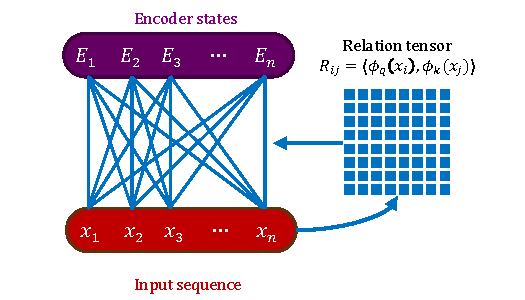
\includegraphics[width=\textwidth]{figures/self_attn_fig.pdf}
        \caption{$E \gets \mathrm{SelfAttention}(X)$}
        \label{fig:self_attention}
    \end{subfigure}
    \hfill
    \begin{subfigure}[b]{0.5\textwidth}
        \centering
        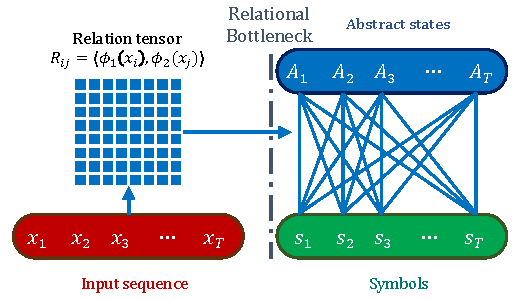
\includegraphics[width=\textwidth]{figures/rel_crossattn_fig.pdf}
        \caption{$A \gets \mathrm{RelationalCrossAttention(X, S)}$}
        \label{fig:relational_cross_attention}
    \end{subfigure}
    \caption{Comparison of relational cross-attention with self-attention. Red represents the sensory information of individual objects, blue represents relational information, and purple represents entangled representations of sensory and relational information. Relational cross-attention computes relational information disentangled from the features of individual objects.}
    \label{fig:attn_mechanisms}
\end{figure}

\subsection{Abstractor module}\label{ssec:abstractor_module}

We now describe the Abstractor module. Like the Encoder in a Transformer, this is a module which processes an input sequence of objects $X = \paren{x_1, \ldots, x_\m}$ producing a a processed sequence of objects $A = \paren{A_1, \ldots, A_\m}$ which represents features of the input sequence. In the Encoder, the output objects $E = \paren{E_1, \ldots, E_\m}$ represents a mix of sensory information about individual objects and relational information. In the Abstractor, $A$ represents purely relational information which is abstracted away from the features of individual objects. The core operation in an Abstractor module is relational cross-attention. Mirroring an encoder, an Abstractor module can consist of several layers, each consisting of relational cross-attention followed by a feedforward network. Optionally, we might apply a residual connection and layer-normalization as suggested in~\citep{vaswani2017attention}. The algorithmic description is presented in~\Cref{alg:abstractor_module}.

\begin{algorithm}[ht!]
	\caption{Abstractor module}\label{alg:abstractor_module}
	\SetKwInOut{Input}{Input}
	% \SetKwInOut{Output}{Output}
	% \SetKwInOut{LearnableParams}{Learnable parameters}
	% \SetKwInOut{HyperParams}{Hyperparameters}

	\Input{object sequence: $\bm{X} = (x_1, \ldots, x_\m) \in \reals^{d \times \m}$ }
	% \HyperParams{Dimension of relation $d_r$, Projection dimension $d_p$, dimension of embedding $d_e$}
	% \LearnableParams{projection matrices $W_1^{(i)}, W_2^{(i)} \in \reals^{d_p \times d_e}, \ i=1, \ldots, d_r$, parameters of feedforward networks}
	\vspace{1em}

    $A^{(0)} \gets S_{1:\m}$

	\For{\(l \gets 1\) \KwTo \(L\)}{

        $A^{(l)} \gets \mathrm{RelationalCrossAttention}\paren{X, A^{(l-1)}}$

        $A^{(l)} \gets A^{(l)} + A^{(l-1)}$ \quad \texttt{residual connection (optional)}

        $A^{(l)} \gets \mathrm{LayerNorm}(A^{(l)})$ \quad \texttt{(optional)}

        $A^{(l)} \gets \mathrm{FeedForward}\paren{A^{(l)}}$

        % \vspace{1em}
        % \texttt{optionally, self-attention:}

        % $A^{(l)} \gets \mathrm{SelfAttention}\paren{A^{(l)}}$

        % $A^{(l)} \gets A^{(l)} + A^{(l-1)}$ \quad \texttt{residual connection (optional)}

        % $A^{(l)} \gets \mathrm{LayerNorm}(A^{(l)})$ \quad \texttt{(optional)}

        % $A^{(l)} \gets \mathrm{FeedForward}\paren{A^{(l)}}$
    }

    \textbf{Output:} $A^{(L)}$

\end{algorithm}

The hyperparamters of an Abstractor module includes the the number of layers $L$, the relation dimension $d_r$ (i.e., number of heads),  the projection dimension $d_p$ (i.e., key dimension), the relation activation function $\sigma_{\mathrm{rel}}$, the dimension of the symbols $d_s$, the parameters of the feedforward network, whether to apply a residual connection, and whether to apply layer-normalization. The learnable parameters, at each layer, are the projection matrices $W_1^{(i)}, W_2^{(i)} \in \reals^{d_p \times d_s}, \ i \in [d_r]$, the symbols $S = \paren{s_1, s_2, \ldots } \in \reals^{d_s \times \texttt{max\_len}}$, and the parameters of the feedforward network. In our experiments, we use a 2-layer feedforward network with a hidden dimension $d_{\mathrm{ff}}$ and ReLU activation. The implementation in the publicly available code includes a few additional hyperparameters including whether to restrict the learned relations to be symmetric (via $W_1^{(i)} = W_2^{(i)}$), and whether to additionally apply self-attention after relational cross-attention. The symbols in the Abstractor can be either learned parameters or nonparametric positional embeddings (e.g., sinusoidal positional embeddings).

Observe that in the first layer of the Abstractor, the values in relational cross-attention are the input-independent symbols. In the following layers, the values are the abstract states from the previous layer. In the next subsection we characterize the function class of 1-layer Abstractor modules. Computations in deeper Abstractor modules are more difficult to interpret in terms of the original input sequence, but, empirically, we find that deeper Abstractor modules can yield improvements in performance.

\begin{remark}[Length generalization]
    Similar to positional embeddings in standard Transformers, the symbols $S = (s_1, s_2, \ldots)$ can be either learned parameters of the model or non-parameteric positional embeddings (e.g., sinusoidal positional embeddings). In principle, using non-parameteric positional embeddings as symbols allows for generalization to longer sequence lengths than was observed during training. However, length-generalization remains an unsolved challenge in Transformers~\citep{kazemnejadImpactPositionalEncoding2023}. Although we don't carry-out a systematic evaluation of length-generalization for Abstractor-based models, it is likely that the same challenges apply. To begin to address this, we propose a variant of the Abstractor which uses position-relative symbols, $S = \paren{\ldots, s_{-1}, s_0, s_1, \ldots}$, where the message-passing operation of relational cross-attention becomes,
    \begin{equation}\label{eq:position_relative_symbols}
        \begin{split}
            A_i &\gets \mathrm{MessagePassing}\paren{\set{(s_{j-i}, R_{ij})}_{j \in [\m]}}\\
            &= \sum_{j} R_{ij} s_{j-i}.
        \end{split}
    \end{equation}

    Hence, the symbols carry information about relative-position with respect to the object being processed, as opposed to absolute position. In Transformers, relative positional embeddings have been shown to yield improvements in length-generalization.
\end{remark}

\subsection{Universal approximation of relation functions for Abstractors}\label{ssec:universal_approximation}

In this section, we consider the representational power of the Abstractor module for computing functions of relations between a sequence of objects. We defer formal statements and proofs to the appendix. We show that the Abstractor module can approximate arbitrary functions of relations between objects, and that the Abstractor module can be composed to compute higher-order relations. Consider a 1-layer single-head Abstractor acting on a sequence of objects $X = \paren{x_1, \ldots, x_\m} \in \calX^\m$. Let $\sigma_\mathrm{rel}$ be the identity. Then, a 1-layer Abstractor computes abstract states as,
\begin{equation}
    A_i \gets \mathrm{FeedForward}\paren{\sum_{j} \iprod{\phi(x_i)}{\psi(x_j)} s_j}.
\end{equation}

The following result shows that a 1-layer Abstractor can approximate arbitrary functions of each object's relations with the other objects. This result follows from the analysis of function classes of inner products of neural networks in~\citep{TODO:POSTtoARXIV}.
\begin{result}\label{result:abstractor_univ_approximation}
    Let $r: \calX \times \calX \to \reals^{d_r}$ be any relation function. Then, there exists a choice of symbols $s_1, \ldots, s_\m$ and parameters of the feed-forward network such that $A_i$ approximates an arbitrary function of $\paren{r(x_i, x_j)}_{j=1}^\m$.
\end{result}

As discussed in the next section, Abstractor modules can be composed in a broader architecture to compute higher-order relations. The following result states that a composition of $k$ single-layer Abstractors can approximate arbitrary $k$th-order relational functions.

\begin{result}\label{result:abstractor_composition}
    A composition of $k$ single-layer Abstractors is able to compute arbitrary $k$th-order relational functions.
\end{result}

Finally, we present a robustness result which states that relational cross-attention is able to encodes relations robustly via redundancy in the symbols.

\begin{result}\label{result:abstractor_robustness}
    Suppose that symbolic message-passing is used to transform a sequence of $m$ symbols, each of dimension $d$. If a fraction $\epsilon$ of the entries of the transformed symbols are arbitrarily corrupted, the relations can be exactly recovered by a linear program as long as $\sqrt{m/(1-\epsilon)^2d}$ is sufficiently small.
\end{result}

The results of~\citep{model_repair} make the robustness properties precise. We investigate different forms of robustness empirically in the experiments section.

\section{Abstractor architectures}\label{sec:abstractor_architectures}

% Similar to a Transformer Encoder, an Abstractor is a module that takes a sequence of objects $X = (x_1, \ldots, x_\m)$ as input and produces a processed representation of the input as another sequence of objects, $A = (A_1, \ldots, A_\m)$. In contrast to the encoder states $E = \paren{E_1, \ldots, E_\m}$, which represent an entangled mixture of object-level attributes and relational information, the abstract states $A$ represent only relational information of the input, abstracted away from the object-level attributes. An Abstractor is a module whose purpose is to process purely relational information. It can be integrated into a broader transformer-based architecture in several different ways, depending on the target task.

Whereas an Encoder performs ``general-purpose'' processing, extracting representations of both object-level and relational information, an Abstractor module is more specialized and produces purely relational representations. An Abstractor can be integrated into a broader transformer-based architecture, for enhanced relational processing.

To facilitate the discussion of different architectures, we distinguish between two types of tasks. In a \textit{purely relational} prediction task, there exists a sufficient statistic of the input which is purely relational and encodes all the information that is relevant for predicting the target. The experiments of~\citep{esbn,kerg2022neural} are examples of discriminative purely relational tasks. An example of a sequence-to-sequence purely relational task is the object-sorting task described in~\Cref{ssec:experiments_object_sorting}. To predict the `argsort' of a sequence of objects, the pairwise $\prec$ relation is sufficient. Many real-world tasks, however, are not purely relational. In a \textit{partially-relational} prediction task, the relational information is important, but it is not sufficient for predicting the target. Natural language understanding is an example of a partially-relational task. The math problem-solving experiments in~\Cref{ssec:experiments_math} are also partially-relational.

\begin{figure}
    \centering
    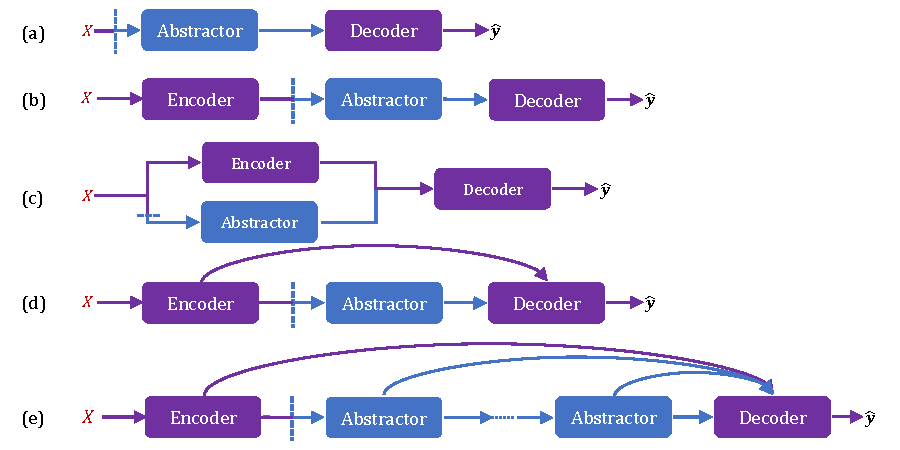
\includegraphics[width=0.9\textwidth]{figures/abstractor_architectures.pdf}
    \caption{Examples of Abstractor-based model architectures.}\label{fig:abstractor_architectures}
    % \vskip-10pt
\end{figure}


The way that an Abstractor module is integrated into a broader model architecture should be informed by the underlying prediction task.~\Cref{fig:abstractor_architectures} depicts several Abstractor architectures each with different properties. Architecture (a) depicts an architecture in which the Abstractor processes the relational features in the input, and the decoder attends to the abstract states $A$. Architecture (b) depicts a model in which the input objects are first processed by an Encoder, followed by an Abstractor for relational processing, and the decoder again attends to the abstract states. These architectures would be appropriate for purely relational tasks since the decoder attends only to the relational representations in the abstract states. Architectures (c) and (d) would be more appropriate for more general tasks which are only partially relational. For example, in architecture (c), the model branches into two parallel processing streams in which an Encoder performs general-purpose processing and an Abstractor performs more specialized processing of relational information.
The decoder attends to \textit{both} the encoder states and abstract states.
% We refer to architectures which combine sensory processing with abstract relational processing as \textit{sensory-connected} architectures.
These architectures use the ``multi-attention decoder'' described in~\Cref{alg:multi_attention_decoder} in the appendix.
Finally, architecture (e) depicts a \textit{composition} of Abstractors, wherein the abstract states produced by one Abstractor module are used as input to another Abstractor. This results in computing ``higher-order'' relational information (i.e., relations on relations).
% This is made formal in~\Cref{ssec:function_classes_preview}. % we cut out the abstractor theory section. hopefully we can include it in a final version?
We leave empirical evaluation of this architecture to future work.


\section{Experiments}\label{sec:experiments}

\footnotetext{\footnotesize We ran the experiments described here on RTX 2080ti, RTX 3090, and A100 GPUs, available to us through our institution's internal cluster. The models here are relatively small; powerful GPUs are not required to train a single model. We found the use of GPUs useful for evaluating learning curves over several trials.}

\subsection{Warm up: Ability to learn asymmetric and multi-dimensional relations}
One recent work on relational machine learning is~\cite{kerg2022neural} where, based on prior work~\cite{esbn}, the
authors argue for a particular type of inductive bias in relational models and propose CorelNet. The architecture is: given a sequence of objects $(x_1, \ldots, x_m)$, embed them using an MLP $\phi$, then compute the similarity matrix $R = \text{Softmax}(A), A = {\left[\langle\phi(x_i), \phi(x_j)\rangle\right]}_{ij}$. The final output is an MLP applied to the flattened similarity matrix. They demonstrate that this model can solve a series of simple tasks with high sample-efficiency compared to models like ESBN and standard Transformers. However, CorelNet has some notable limitations. One is that, as described,
it is only able to model symmetric relations\footnote{This is not fundamental to the CoRelNet model, which can learn asymmetric relations via the natural modification $A = {\left[\langle W_1 \phi(x_i), W_2 \phi(x_j)\rangle\right]}_{ij}$, where $W_1, W_2$ are trainable matrices.}---$R$ is symmetric by definition.
Another limitation is that it can only model single-dimensional relations---for each pair of objects $(i,j)$, their modeled relation is a single-dimensional scalar $R_{ij}$. The Abstractor is able to model a significantly larger class of relations. In particular, it is able to model asymmetric and multi-dimensional relations through the $\text{MultiHeadRelation}$ operation. This is demonstrated by the following simple experiment. Note that this is merely intended as a warm up; we don't wish to imply that this task is not solvable by standard models which lack a relational bottleneck (see the following experiments for more interesting comparisons).

We generate $N = 32$ ``random objects'' represented by iid Gaussian vectors, $o_i \overset{iid}{\sim} \mathcal{N}(0,
I_d) \in \mathbb{R}^d$, and associate an order relation to them $o_1 \prec o_2 \prec \cdots \prec o_N$. We train
several different relational models to learn this order relation. Note that $\prec$ is \textit{not symmetric}. Of the $N^2 = 1024$ possible pairs $(o_i, o_j)$, 15\% are held out as a validation set (for early stopping) and 35\% as a test set. We evaluate learning curves by training on the remaining 50\% and computing accuracy on the test set (10 trials for each training set size). Note that under this set up, we are evaluating the models on pairs they have never seen. Thus, the models will need to generalize based on the transitivity of the $\prec$ relation. We observe that a simple Abstractor model is able to learn the relation while CorelNet cannot~(\Cref{fig:exp_order_relation}).

For completeness, we also compare to a standard Transformer model. The transformer model performs slightly better than the Abstractor on this simple task. We include this to highlight that an Abstractor will not necessarily be superior to a Transformer uniformly on all tasks, but rather that it can realize significant gains on tasks with complex relational structure (see the following experiments).

\begin{figure*}
    \vskip-.2in
    \begin{subfigure}[t]{0.40\textwidth}
        %\centering
        \hskip-.35in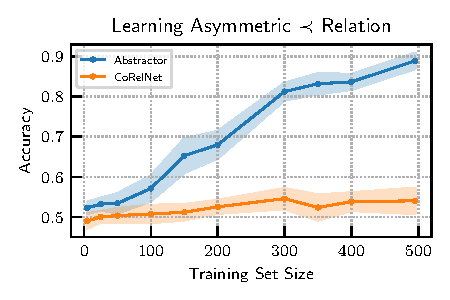
\includegraphics[scale=.95]{figures/experiments/pairwise_order_learning_curves.pdf}
        \vskip-5pt
        \caption{The Abstractor learns the transitive $\prec$ relation and generalizes, whereas CorelNet's learning curve is flat at the baseline accuracy of 0.5.}\label{fig:exp_order_relation}
    \end{subfigure} \hspace{\fill}
    \captionsetup[subfigure]{oneside,margin={-.3in,0in}}
    \begin{subfigure}[t]{0.40\textwidth}
        %\centering
        % \vskip10pt
        \hskip-.6in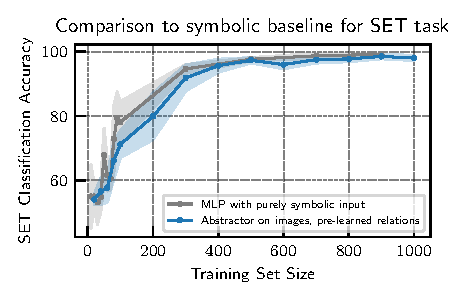
\includegraphics[scale=.95]{figures/experiments/set_symbolic_vs_abstractor.pdf}
        \vskip-5pt
        \caption{Comparison of Abstractor trained on images of cards and MLP with relations hand-encoded symbolically as bit vectors.}% The Abstractor is nearly as sample efficient as symbolic computation.}
        \label{fig:exp_set}
    \end{subfigure}

    \begin{subfigure}[t]{0.40\textwidth}
        %\centering
        \hskip-.35in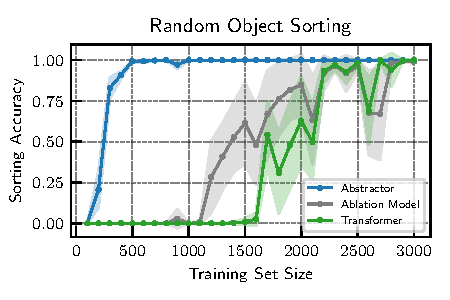
\includegraphics[scale=.95]{figures/experiments/random_object_sorting.pdf}
        \vskip-5pt
        \caption{Learning curves on sorting sequences of random objects. The abstractor is dramatically more sample-efficient.}\label{fig:exp_object_sorting}
    \end{subfigure}\hspace{\fill}
    \begin{subfigure}[t]{0.40\textwidth}
        %\centering
        \hskip-.6in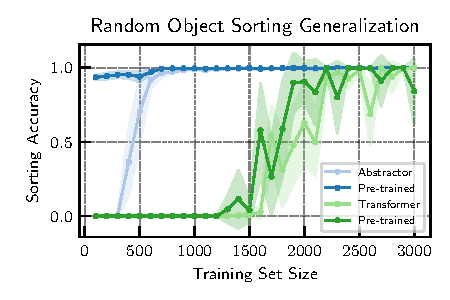
\includegraphics[scale=.95]{figures/experiments/random_object_sorting_generalization.pdf}
        \vskip-5pt
        \caption{Learning curves with and without pre-training on a similar sorting task. The Abstractor benefits significantly from pre-training.}\label{fig:exp_object_sorting_generalization}
    \end{subfigure}
    % \bigskip

    \begin{subfigure}[t]{0.40\textwidth}
        %\centering
        \hskip-.35in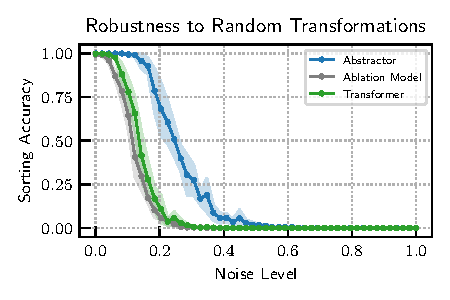
\includegraphics[scale=.95]{figures/experiments/additive_robustness.pdf}
        \vskip-5pt
        \caption{The Abstractor is more robust to corruption by additive noise. }\label{fig:exp_robustness}
    \end{subfigure}\hspace{\fill}
    \begin{subfigure}[t]{0.40\textwidth}
        %\centering
        \hskip-.6in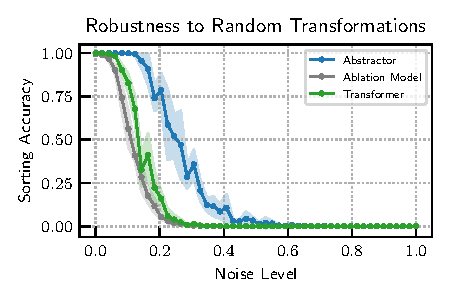
\includegraphics[scale=.95]{figures/experiments/multiplicative_robustness.pdf}
        \vskip-5pt
        \caption{The Abstractor is more robust to corruption by a random linear transformation.}\label{fig:exp_robustness2}
    \end{subfigure}

    \caption{Experiments. Shaded regions indicate twice the standard error of mean.}\label{fig:experiments}
    \vskip-.10in
\end{figure*}

\subsection{Superior sample-efficiency on relational tasks compared to plain transformers}
The next experiment extends the idea of learning an order relation $\prec$ on random objects: now, the task is to fully sort sequences of randomly permuted random objects.

We generate random objects in the following way. First, we generate two sets of random attributes $\mathcal{A} = \{a_1, a_2, a_3, a_4\}$, $a_i \overset{iid}{\sim} \mathcal{N}(0, I) \in \mathbb{R}^{4}$ and $\mathcal{B} = \{b_1, \ldots, b_{12}\}$, $b_i \overset{iid}{\sim} \mathcal{N}(0, I) \in \mathbb{R}^{8}$. To each set of attributes, we associate the strict ordering relation $a_1 \prec a_2 \prec a_3 \prec a_4$ and $b_1 \prec b_2 \prec \cdots \prec b_{12}$, respectively. Our random objects are formed by the Cartesian product of these two attributes $\mathcal{O} = \mathcal{A} \times \mathcal{B}$, yielding $N = 4 \times 12 = 48$ objects (i.e., each object in $\mathcal{O}$ is a vector in $\mathbb{R}^{4+8}$ formed by a concatenation of one attribute value in $\mathcal{A}$ and one in $\mathcal{B}$). Then, we associate with $\mathcal{O}$ the strict ordering relation corresponding to the order relation of $\mathcal{A}$ as the primary key and the order relation of $\mathcal{B}$ as the secondary key. i.e., $(a_i, b_j) \prec (a_k, b_l)$ if $a_i \prec a_k$ or if $a_i = a_k$ and $b_j \prec b_l$.

Given a set of objects in $\mathcal{O}$, the task is to sort it according to $\prec$. More precisely, the input sequences are randomly permuted sequences of $10$ objects in $\mathcal{O}$ and the target sequences are the indices of the object sequences in sorted order (i.e., the `argsort'). The training data are sampled uniformly from the set of length-10 sequences in $\mathcal{O}$. We also generate a non-overlapping validation dataset (used during training for early stopping) and a testing dataset (used during evaluation).

We evaluate learning curves on an Abstractor, a Transformer, and an ``Ablation'' model (10 trials for each training set size). The Abstractor uses the architecture $\texttt{Encoder} \to \texttt{Abstractor} \to \texttt{Decoder}$. The Encoder-to-Abstractor interface uses relational cross-attention and the Abstractor-to-Decoder interface uses standard cross-attention. The Ablation Model aims to test the effects of the relational cross-attention in the Abstractor model---it is architecturally identical to the Abstractor model with the crucial exception that the Encoder-to-Abstractor interface instead uses standard cross-attention. The hyperparameters of the models are chosen so that the parameter counts are similar. % TODO: add details here? or in supplement?
We find that the Abstractor is dramatically more sample-efficient than the Transformer and the Ablation model~(\Cref{fig:exp_object_sorting}).

\subsection{Ability to generalize to similar tasks}

Continuing with the object-sorting task and the dataset generated as described above, we test the Abstractor's ability to generalize from similar relational tasks through pre-training. The main task uses the same dataset described above. The pre-training task involves the same object set $\mathcal{O}$ but the order relation is changed. The ordering in attribute $\mathcal{A}$ is randomly permuted, while the ordering in attribute $\mathcal{B}$ is kept the same. A strict ordering relation $\prec$ on $\mathcal{O}$ is obtained in the same way---using the order in $\mathcal{A}$ as the primary key and the order in $\mathcal{B}$ as the secondary key.

The Abstractor model here uses the architecture $\texttt{Abstractor} \to \texttt{Decoder}$ (i.e., no Transformer
encoder), and the transformer is the same as the previous section. We pre-train both models on the pre-training task
and then, using those learned weights for initialization, evaluate learning curves on the original task. Since the
Transformer requires more training samples to learn the object-sorting task, we use a pre-training set size of $3,000$, chosen based on the results of the previous subsection so that it is large enough for the Transformer to learn the pre-training task. This experiment assesses the models' ability to generalize relations learned on one task to a new task.~\Cref{fig:exp_object_sorting_generalization} shows the learning curves for each model with and without pre-training. We observe that when the Abstractor is pre-trained, its learning curve on the object-sorting task is significantly accelerated. The transformer does not benefit from pre-training.

\subsection{Robustness and Out-of-Distribution generalization}
In this experiment, we evaluate robustness to a particular type of noisy corruption. We train each model on the same
object-sorting task described above. We use a fixed training set size of $3,000$ for the same reason
---it is large enough that all models are able to learn the task. On the hold out test set, we corrupt the object
representations by applying a random linear transformation. In particular, we randomly sample a random matrix the
entries of which are iid zero-mean Gaussian with variance $\sigma^2$, $\Phi \in \mathbb{R}^{d \times d}, \Phi_{ij} \sim \mathcal{N}(0, \sigma^2)$. Each object in $\mathcal{O}$ is then corrupted by this random linear transformation,
$\tilde{o}_i = \Phi o_i, \ \text{ for each } i \in [48]$. We also test robustness to additive noise via $\tilde{o}_i = o_i + \varepsilon_i, \varepsilon_i \sim \mathcal{N}(0, \sigma^2 I_d)$.

The models are evaluated on the hold-out test set with objects replaced by their corrupted version. We evaluate the sorting accuracy of each model while varying the noise level $\sigma$ (5 trials at each noise level). The results are shown in figures~\ref{fig:exp_robustness} and~\ref{fig:exp_robustness2}. We emphasize that the models are trained only on the original objects in $\mathcal{O}$, and are not trained on objects corrupted by any kind of noise.

This experiment can be interpreted in two lights: the first is robustness to noise. The second is a form of out-of
-distribution generalization. Note that the objects seen by the models post-corruption lie in a different space than
those seen during training. Hence the models need to learn relations that
are in some sense independent of the value representation.
As a theoretical justification for this behavior,~\cite{zhouCompressedPrivacySensitive2009} shows that $\langle \Phi x, \Phi y \rangle \approx \langle x, y \rangle$ in high dimensions, for a random matrix $\Phi$ with iid Gaussian entries. This indicates that models whose primary computations are performed via inner products, like Abstractors, may be more robust to this kind of corruption.

\subsection{Modularity and comparison to purely symbolic representations}
\label{ssec:set_exp}


\begin{wrapfigure}{R}{0.25\textwidth}
	\vskip-5pt
	\begin{tabular}{c}
		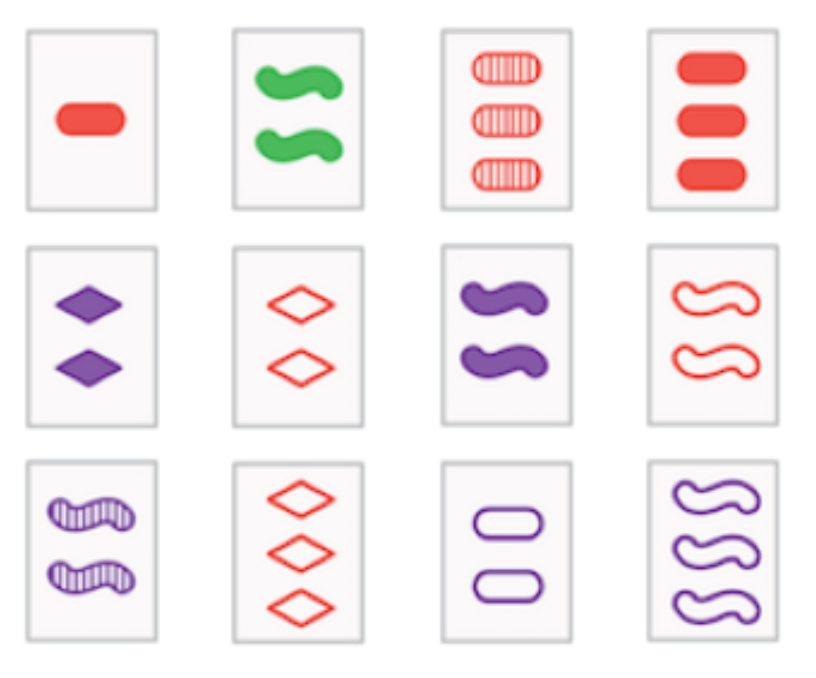
\includegraphics[width=.25\textwidth]{figures/set_example}\\[-5pt]
	\end{tabular}
	\caption{\footnotesize The SET game}
\end{wrapfigure}
SET is a relatively straightforward but challenging cognitive task that engages reasoning faculties in a deliberative
, attentionally directed manner, requiring several levels of abstraction over sensory embeddings. Players are
presented with 12 cards, each of which contains figures that vary along four dimensions (color, number, pattern, and
shape) and they must find subsets of three cards which obey a deceptively simple rule: along each dimension, all cards in a SET must either have the same or unique values.
% JDC: DO FIGURES NEED TO BE NUMBERED?
For example, in the figure to the right, the cards with two solid blue/purple diamonds, two striped blue squiggles, and two open blue oblongs form a SET: same color, same number, different patterns, different shapes.

To simulate the task of deciding if a triple forms a SET, we first train a convolutional neural network to process the color images of the cards (a full deck includes 81 cards). The CNN is trained to predict the attribute of
each card, as a multi-label classification, and then an embedding of dimension $d=32$ of 
each card is obtained. This embedding layer uses an \MLP{} to map the convolutional feature maps into a distributed
representation. Next, we train Abstractors separately for each of the four attributes to learn same/different
relations, where the task is to decide if an input pair of cards is the same or different for that attribute. 
We then use the query and key mappings $W_Q$ and $W_K$ learned for these relations to initialize the relations
in a multi-head Abstractor. The Abstractor is then trained on a dataset of triples of cards, half of which form a SET. 

This is compared to a baseline symbolic model where, instead of images, the input is a vector with 12 bits,
explicitly encoding the relations. That is, for each of the four attributes, a binary symbol is computed for each pair of three input cards---1 if the pair is the same in that attribute, and 0 otherwise. A two-layer MLP is then trained to decide if the triple forms a SET. The MLP using the symbolic representation can be considered as a lower bound on the performance achievable by the Abstractor. This comparison shows that the Abstractor is able to solve a task using relations learned in other tasks (modularity), with a sample efficiency that is not far from that obtained
with purely symbolic, noise-free encodings of the relevant relations. %We note that this uses a simple Abstractor configuration, without self-attention.

% JDC: I REALIZE WE ARE TIGHT ON SPACE, BUT IF THERE IS ROOM, COULD ADD THE FOLLOWING, OR A SHORTENED FORM OF
This subtask suggets how Abstractors might be viewed as an intermediate between strong ``nativist'' approaches that assume a pre-existing foundation of symbolic primitives and purely ``empiricist'' approaches that assume
similar capabilities can emerge simply from processing large amounts of data \cite{howtogrowamind}.
%can be achieved simply by the application of general purpose learning algorithms to large
%amounts of data -- showing how the latter, agumented with simple architectural inductive biases and trained using
%plausible and practical forms of curricular learninng both to generate genuinely symbolic representations, and use these to achieve the flexibilty and efficiency characteristic of human reasoning.
\footnote{We ran the experiments described here on RTX 2080ti, RTX 3090, and A100 GPUs which we had available to us via our institute's internal cluster. The models here are relatively small; powerful GPUs are not required to train a single model. We found the use of GPUs useful for evaluating learning curves over several trials.}
\section{Discussion}\label{sec:discuss}

% In this work we have proposed a framework which extends Transformer models to naturally support types of relational learning, through a cross-attention mechanism that enforces a relational bottleneck, separating relational information from object-level attributes. Building on insights gained from the implementation of a relational bottleneck in other forms \citep{esbn, kerg2022neural}, this exploits the powerful attentional capabilities of the transformer architecture to identify relevant relationships. Our experiments validate that the proposed architecture enables dramatic improvements in relational processing, and that this has the potential to translate into meaningful gains in more general sequence modeling tasks.
% % Experiments with controlled purely relational tasks as well as more general sequence modeling tasks indicate that this framework has the potential to combine the benefits of function approximation over sensory states, as exploited in many deep learning models, with abstraction and relational reasoning abilities supported by symbolic processing.
% Interesting work remains to better understand the potential of this framework, and how it may relate to the algorithms of human cognition as implemented in the brain.

In this work, we propose a variant of attention that produces representations of relational information disentangled from object-level attributes. This leads to the development of the Abstractor module, which fits naturally into the powerful framework of Transformers. Through a series of experiments, we demonstrate the potential of this new framework to achieve gains in sample efficiency in both purely relational tasks and more general sequence modeling tasks.

This work opens up several avenues for future research. One possible line of research is to better understand the role of symbols within the Abstractor, including the trade-offs between learned symbols, parametric symbols, and the use of position-relative symbols. Another important line of research is the study of the alternative architectural variants proposed in~\Cref{fig:abstractor_architectures}. In particular, understanding the properties of compositions of Abstractor modules and assessing such an architecture's ability to represent higher-order relations will shed light on the expressive power of the framework. Finally, the experiments presented here demonstrate the Abstractor's promise and utility for relational representation in Transformers, and it will be interesting to explore the framework's use in increasingly complex modeling problems. 

\subsection*{Code and Reproducibility}
Code, detailed experimental logs, and instructions for reproducing our experimental results are available at: \url{https://github.com/Awni00/Abstractor}.

% !TEX root = ./repair.tex

\section*{Acknowledgments}

Research supported in part by NSF grant CCF-1839308 and a 
Vannevar Bush Faculty Fellowship to JC.


\printbibliography
% \bibliography{references}
% \bibliographystyle{iclr2024_conference}

\clearpage
\appendix
\section{Multi-Attention Decoder}\label{sec:multi_attn_decoder}

\begin{algorithm}[ht!]
	\caption{Multi-Attention Decoder}\label{alg:multi_attention_decoder}
	\SetKwInOut{Input}{Input}
	% \SetKwInOut{Output}{Output}
	% \SetKwInOut{LearnableParams}{Learnable parameters}
	% \SetKwInOut{HyperParams}{Hyperparameters}

	\Input{
        Target sequence: $\bm{y} = (y_0, \ldots, y_{l_y-1})$, \\
        Context sequences: $X^{(i)} = (x_1^{(i)}, \ldots, x_{l_i}^{(i)}), \ i=1, \ldots, K$
        }
	\vspace{1em}

    $D^{(0)} \gets \bm{y}$

	\For{\(l \gets 1\) \KwTo \(L\)}{

        $D^{(l)} \gets \mathrm{CausalSelfAttention}\paren{D^{(l-1)}}$

        \texttt{residual connection and layer-normalization}


        \For{\(i \gets 1\) \KwTo \(K\)}{
            $D^{(l)} \gets \mathrm{CrossAttention}\paren{D^{(l)}, X^{(i)}}$

            \texttt{residual connection and layer-normalization}
        }

        $D^{(l)} \gets \mathrm{FeedForward}\paren{D^{(l)}}$

        }

    \textbf{Output:} $D^{(L)}$

\end{algorithm}

\section{Universal approximation of relation functions}\label{sec:abstractor_approx_theory}

In this section, we characterize the function class of the Abstractor and relational cross-attention. Recall that relational cross-attention takes the form
\begin{equation*}
    A \gets S \sigma_{\mathrm{rel}}\paren{\phi(X)^\top \psi(X)},
\end{equation*}
where $\phi, \psi: \calX \to \reals^{d_{\mathrm{proj}}}$ are multi-layer perceptrons, and $S$ is the matrix of symbols. In this analysis, we consider $\sigma_{\mathrm{rel}}: x \mapsto x$ to be the linear activation function. Further, we consider positional symbols. For simplicity, we will assume the single-head variant of relational cross-attention. The function class results derived here would of course carry over to the multi-head case, where each `head' can approximate a function in the function class.

Recall that an Abstractor module comprises several layers, each composed of relational cross-attention and a feedforward layer. Hence, the overall operation in one layer of an Abstractor module is
\begin{equation}\label{eq:abstractor_layer}
    \mathrm{AbstractorLayer}(X) = \mathrm{FeedForward}\paren{S\, \phi(X)^\top \psi(X)}.
\end{equation}
We will characterize the function class $\mathrm{AbstractorLayer}: \calX^n \to \reals^{d \times n}$ induced by varying the parameters of $\phi,\, \psi,\, \mathrm{FeedForward}$ and $S$.

\begin{remark}
    In~\Cref{eq:relational_crossattn}, we formulate relational cross-attention with the maps $\phi, \psi$ as linear projections, whereas $\phi, \psi$ are multi-layer perceptrons in~\Cref{eq:abstractor_layer}. However, recall that the input to each Abstractor layer is the output of the preceding layer which ends with a multi-layer perceptron. The function class of a multi-layer perceptron followed by two different linear projections is the same as the function class of two different multi-layer perceptrons. We focus on~\Cref{eq:abstractor_layer} for ease of presentation.
\end{remark}

The following result shows that a single-layer abstractor returns a sequence of abstract states which can approximate an arbitrary function of each object's relations with the other object in the input. The result is based on the analysis in~\citep{altabaaApproximationRelationFunctions2024} which characterizes the function class of inner products of neural networks.

\begin{theorem}
    Suppose $\calX$ is a compact euclidean space. Let $r: \calX \times \calX \to \reals$ be any continuous relation function, and $f: \reals^n \to \reals^d$ any continuous function. Consider the function $g: \calX^n \to \reals^{d \times n}$ defined by
    \begin{equation*}
        (x_1, \ldots, x_n) \mapsto \paren{f(R_1), \ldots, f(R_n)},
    \end{equation*}
    where $R_i = {(r(x_i, x_j))}_{j \in [n]}$ is the vector of $x_i$'s relations with the other objects in the input, according to $r$. Then, for any $\varepsilon > 0$, there exists MLPs $\phi, \psi, \mathrm{FeedForward}$ and a choice of symbols $S$ such that the Abstractor layer approximates $g$ in the sup-norm
    \begin{equation*}
        \infnorm{g(x_1, \ldots, x_n) - \mathrm{AbstractorLayer}(x_1, \ldots, x_n)} \leq \varepsilon, \quad \text{Lebesgue almost-everywhere.}
    \end{equation*}
\end{theorem}
\begin{proof}
    Let $(A_1, \ldots, A_n) = \mathrm{AbstractorLayer}(x_1, \ldots, x_n)$ be the abstract states returned by the abstractor layer. For each $i \in [n]$,
    the abstract state $A_i$ takes the form,
    \begin{equation*}
        A_i = \mathrm{FeedForward}\paren{\sum_{j=1}^{n} \iprod{\phi(x_i)}{\psi(x_j)} s_j}.
    \end{equation*}
    where $S = (s_1, \ldots, s_n)$ are the symbols assigned to each object. Let the symbol dimension be $n$ and let $s_i = \bm{e}_i$, the canonical basis vectors. Then, $A_i = \mathrm{FeedForward}(R_i)$, where $R_i = {(\iprod{\phi(x_i)}{\psi(x_j)})}_{j \in [n]} \in \reals^n$. By~\citep[Theorem 3.1]{altabaaApproximationRelationFunctions2024}, there exists MLPs $\phi, \psi$ such that their inner product approximates any continuous relation function. In particular, for any $\varepsilon_1 > 0$, there exists $\phi, \psi$ such that
    \begin{equation}\label{eq:approx_proof_r_approx}
        \abs{r(x, y) - \iprod{\phi(x)}{\psi(y)}} \leq \varepsilon_1, \quad \text{Lebesgue almost-every } x,y \in \calX
    \end{equation}
    Let $\phi, \psi$ be such MLPs where $\varepsilon_1$ is to be determined later. Note that~\citep{altabaaApproximationRelationFunctions2024} gives a bound on the number of neurons needed in terms of the continuity of $r$ and the dimension of $\calX$. Similarly, by the universal approximation property of MLPs~\citep[e.g.,]{cybenkoApproximationSuperpositions1989}, $f: \reals^{n} \to \reals^{d}$ can be approximated by $\mathrm{FeedForward}$ uniformly in the sup-norm. That is, for any $\varepsilon_2$ there exists $\mathrm{FeedForward}$ such that
    \begin{equation}\label{eq:approx_proof_f_approx}
        \sup_{z \in \reals^n} \infnorm{f(z) - \mathrm{FeedForward}(z)} \leq \varepsilon_2.
    \end{equation}

    Let $[R]_{ij} = r(x_i, x_j)$ and $[\hat{R}]_{ij} = \iprod{\phi(x_i)}{\psi(x_j)}$. Then, the difference $g(x_1, \ldots, x_n) - \mathrm{AbstractorLayer}(x_1, \ldots, x_n)$ is given by
    \begin{equation}\label{eq:approx_proof_diff}
        \Big[f(R_{1\cdot}), \ldots, f(R_{1\cdot})\Big] - \Big[\mathrm{FeedForward}(\hat{R}_{1\cdot}), \ldots, \mathrm{FeedForward}(\hat{R}_{n\cdot})\Big]
    \end{equation}

    Note that $\hat{R}_{i\cdot}$ is close to $R_{i\cdot}$ by~\Cref{eq:approx_proof_r_approx}
    \begin{equation}\label{eq:approx_proof_R_approx}
        \begin{split}
            \infnorm{\hat{R}_{i\cdot} - R_{i\cdot}} &= \max_{j \in [n]} \abs{\iprod{\phi(x_i)}{\psi(x_j)} - r(x_i, x_j)} \\
            &\leq \varepsilon_1 \quad \text{Lebesgue almost-everywhere}.
        \end{split}
    \end{equation}

    Now consider the $(i,j)$-th element of the difference in~\Cref{eq:approx_proof_diff}
    \begin{equation*}
        \abs{\mathrm{FeedForward}_i(\hat{R}_{j\cdot}) - f_i(R_{j\cdot})} \leq \abs{\mathrm{FeedForward}_i(\hat{R}_{j\cdot}) - f_i(\hat{R}_{j\cdot})} + \abs{f_i(\hat{R}_{j\cdot}) - f_i(R_{j\cdot})}
    \end{equation*}
    The first term is bounded by $\varepsilon_2$ due to~\Cref{eq:approx_proof_f_approx}. Let $\varepsilon_2 = \varepsilon / 2$. Recall that $f: \reals^n \to \reals^d$ is continuous, and hence for all $\epsilon > 0$ there exists $\delta_f(\varepsilon) > 0$ such that $\infnorm{z_1 - z_2} \leq \delta(\varepsilon) \implies \infnorm{f(z_1) - f(z_2)} \leq \varepsilon$. Letting $\varepsilon_1 = \delta(\varepsilon / 2)$, implies that the second term is bounded by $\varepsilon / 2$ Lebesgue almost-everywhere due to~\Cref{eq:approx_proof_R_approx}.

    This holds for all $i, j$, which completes the proof.

\end{proof}
\section{Experimental details}\label{sec:experimental_details}

In this section, we give further experimental details including architectures, hyperparameters, and implementation details. All model and experiments are implemented in Tensorflow. The code is publicly available on the project repo along with detailed experimental logs and instructions for reproducing our results.

\subsection{Discriminative tasks (\Cref{ssec:experiments_discriminative})}

\subsubsection{Pairwise Order}
\textbf{Abstractor architecture} number of layers $L = 1$, relation dimension $d_r = 4$, symbol dimension $d_s = 64$, projection dimension $d_p = 16$, feedforward hidden dimension $d_{\mathrm{ff}} = 64$, relation activation function $\sigma_{\mathrm{rel}} = \mathrm{sigmoid}$. No layer normalization or residual connection. Positional symbols are used  and are learned parameters of the model.

\textbf{CoRelNet Architecture} Given a sequence of objects, $X = (x_1, \ldots, x_\m)$, standard CoRelNet simply computes the inner product and takes the Softmax. We also add a learnable linear map, $W \in \reals^{d \times d}$. Hence, $\bar{R} = \text{Softmax}(R), R = {\left[\langle W x_i, W x_j\rangle\right]}_{ij}$. The asymmetric variant of CoRelNet is given by $\bar{R} = \text{Softmax}(R), R = {\left[\langle W_1 x_i, W_2 x_j\rangle\right]}_{ij}$, where $W_1, W_2 \in \reals^{d \times d}$ are learnable matrices.

\textbf{Training/Evaluation} We use the sparse categorical crossentropy loss and the Adam optimizer with a learning rate of $10^{-2}$, $\beta_1 = 0.9, \beta_2 = 0.999, \varepsilon = 10^{-7}$. We use a batch size of 64. We train for 100 epochs and restore the best model according to validation loss. We evaluate on the test set.

\subsubsection{SET}

The card images are RGB images of dimension $70 \times 50$. The CNN embedder produces embeddings fo dimension $d=64$ for each card. The CNN is trained to predict the four attributes of each card and then an embedding for each card is obtained from an intermediate layer (i.e., the parameters of the CNN are then frozen). Recall that the common architecture is $\texttt{CNN Embedder} \to \{\texttt{Abstractor} \text{ or } \texttt{CoRelNet}\} \to \texttt{Flatten} \to \texttt{Dense(2)}$. We tested against the standard version of CorelNet, but found that it did not learn anything. We iterated over the hyperparameters and architecture to improve its performance. We found that removing the softmax activation in CoRelNet improved performance a bit. We describe hyperparameters below.

\textbf{Common embedder's architecture} The architecture is given by \texttt{Conv2D} $\to$ \texttt{MaxPool2D} $\to$ \texttt{Conv2D} $\to$ \texttt{MaxPool2D} $\to$ \texttt{Flatten} $\to$ \texttt{Dense(64, 'relu')} $\to$ \texttt{Dense(64, 'relu')} $\to$ \texttt{Dense(2)}. The embedding is extracted from the penultimate layer. The CNN is trained to predict the four attributes of each card until it reaches perfect accuracy and near-zero loss.

\textbf{Abstractor architecture}
The Abstractor module has hyperparameters: number of layers $L = 1$, relation dimension $d_r = 4$, symmetric relations (i.e., $W_1^{(i)} = W_2^{(i)}$, $i \in [d_r]$), linear relation activation (i.e., $\sigma_{\mathrm{rel}}: x \mapsto x$), symbol dimension $d_s = 64$, projection dimension $d_p = 16$, feedforward hidden dimension $d_{\mathrm{ff}} = 128$, and no layer normalization or residual connection. Positional symbols are used  and are learned parameters of the model.

\textbf{CoRelNet Architecture} Standard CoRelNet is described above. It simply computes, $R = \text{Softmax}(A), A = {\left[\langle W x_i, W x_j\rangle\right]}_{ij}$. This variant was stuck at 50\% accuracy regardless of training set size. We found that removing the Softmax helped.~\Cref{fig:exp_set_classification} compares against both variants of CoRelNet.

This finding suggests that allowing $\sigma_{\mathrm{rel}}$ to be a configurable hyperparameter is a useful feature of the Abstractor. Softmax performs contextual normalization of relations, such that the relation between $i$ and $j$ is normalized in terms of $i$'s relations with all other objects. This may be useful at times, but may also cripple a relational model when it is more useful to represent an absolute relation between a pair of objects, independently of the relations with other objects.

\textbf{Data generation} The data is generated by randomly sampling a SET with probability 1/2 and a non-SET with probability 1/2. The triplet of cards is then randomly shuffled.

\textbf{Training/Evaluation} We use the sparse categorical crossentropy loss and the Adam optimizer with a learning rate of $10^{-3}$, $\beta_1 = 0.9, \beta_2 = 0.999, \varepsilon = 10^{-7}$. We use a batch size of 64. We train for 200 epochs and restore the best model according to validation loss. We evaluate on the test set.


\subsection{Relational sequence-to-sequence tasks (\Cref{ssec:experiments_object_sorting})}

\subsubsection{Sample-efficiency in relational seq2seq tasks}

\textbf{Abstractor architecture} The Abstractor model uses architecture (b) of~\Cref{fig:abstractor_architectures}. For each of the Encoder, Abstractor, and Decoder modules, we use 2 layers, 2 attention heads/relation dimensions, a feedforward network with 64 units and an embedding/symbol dimension of 64. The relation activation function is $\sigma_{\mathrm{rel}} = \mathrm{Softmax}$. Positional symbols are used  and are learned parameters of the model. The number of trainable parameters is $386,954$.

\textbf{Transformer architecture} We implement the standard Transformer of~\citep{vaswani2017attention}. For both the Encoder and Decoder modules, we use 4 layers, 2 attention heads, a feedforward network with 64 units and an embedding dimension of 64. The number of trainable parameters is $469,898$. We increased the number of layers compared to the Abstractor in order to make it a comparable size in terms of parameter count. Previously, we experimented with identical hyperparameters (where the Transformer would have fewer parameters due to not having an Abstractor module).

\textbf{Ablation model architecture} The Ablation model uses an identical architecture to the Abstractor, except that the relational cross-attention is replaced with standard cross attention at the Encoder-Abstractor interface (with $Q \gets A, K \gets E, V \gets E$). It has the same number of parameters as the Abstractor-based model.

\textbf{Training/Evaluation} We use the sparse categorical crossentropy loss and the Adam optimizer with a learning rate of $10^{-3}$, $\beta_1 = 0.9, \beta_2 = 0.999, \varepsilon = 10^{-7}$. We use a batch size of 512. We train for 100 epochs and restore the best model according to validation loss. We evaluate learning curves by varying the training set size and sampling a random subset of the data at that size. Learning curves are evaluated starting at 100 samples up to 3000 samples in increments of 100 samples. We repeat each experiment 10 times and report the mean and standard error of the mean.

\subsubsection{Generalization to new object-sorting tasks}

\textbf{Abstractor architecture} The Abstractor model uses architecture (a) of~\Cref{fig:abstractor_architectures}. The Abstractor module uses learned positional symbols, has 1 layer, a symbol dimension of 64, a relation dimension of 4, a softmax relation activation, and a 64-unit feedforward network.  The decoder also has 1 layer with 4-head MHA and a 64-unit feedforward network.

\textbf{Transformer architecture} The Transformer is identical to the previous section.

\textbf{Training/Evaluation} The loss, optimizer, batch size, and learning curve evaluation steps are identical to the previous sections. Two object-sorting datasets are created based on an ``attribute-product structure''---an primary dataset and a pre-training dataset. As described in~\Cref{ssec:experiments_object_sorting}, the pre-training dataset uses the same random objects as the primary dataset but with the order relation of the primary attribute reshuffled. The models are trained on 3,000 labeled sequences of the pre-training task and the weights are used to initialize training on the primary task. Learning curves are evaluated with and without pre-training for each model.

\subsection{Math Problem-Solving (\Cref{ssec:experiments_math})}

\textbf{Abstractor architectures.} The Abstractor models use architecture (d) of~\Cref{fig:abstractor_architectures}. The Encoder, Abstractor, and Decoder modules share the same hyperparameters: number of layers $L = 1$, relation dimension/number of heads $d_r = n_h = 4$, symbol dimension/model dimension $d_s = d_{\mathrm{model}} = 128$, projection dimension $d_p = 32$, feedforward hidden dimension $d_{\mathrm{ff}} = 256$. In the Abstractor, the relation activation function is $\sigma_{\mathrm{rel}} = \mathrm{softmax}$. In one model, positional symbols are used, with sinusoidal embeddings. In the other model, symbolic attention is used with a symbol library of $n_s = 256$ learned symbols, and $4$-head cross-attention.

\textbf{Transformer architecture.} The Transformer Encoder and Decoder have identical hyperparameters to the Encoder and Decoder of the Abstractor architecture.

\textbf{Transformer+ architecture.} In `Transformer+', the model dimension is increased to $d_\mathrm{model} = 200$ and the feedforward hidden dimension is increased to $d_{\mathrm{ff}} = 400$. The remaining hyperparameters are the same.

\textbf{Training/Evaluation} We train each model for 50 epochs with the categorical cross-entropy loss and the Adam optimizer using a learning rate of $6 \times 10^{-4}$, $\beta_1 = 0.9, \beta_2 = 0.995, \varepsilon = 10^{-9}$. We use a batch size of 128.

\subsection{Additional Experiment: Robustness and Out-of-Distribution generalization in the Object-Sorting Experiments}

\subsection{Object-sorting: Robustness and Out-of-Distribution generalization}

This experiment explores the Abstractor's robustness to noise and out-of-distribution generalization as compared to a standard Transformer. We consider the models in~\Cref{ssec:experiments_object_sorting} and the corresponding object-sorting task. We train each model on this task using 3,000 labeled sequences. We choose the fixed training set size of 3,000 because is large enough that both the Abstractor and Transformer are able to learn the task. Then, we corrupt the objects with noise and evaluate performance on sequences in the hold-out test set where objects are replaced by their corrupted versions. We evaluate robustness to a random linear map as well as to additive noise, while varying the noise level. We evaluate over several trials, averaging over the realizations of the random noise.

On the hold out test set, we corrupt the object representations by applying a random linear transformation. In particular, we randomly sample a random matrix the entries of which are iid zero-mean Gaussian with variance $\sigma^2$, $\Phi \in \mathbb{R}^{d \times d}, \Phi_{ij} \sim \mathcal{N}(0, \sigma^2)$. Each object in $\mathcal{O}$ is then corrupted by this random linear transformation, $\tilde{o}_i = \Phi o_i, \ \text{ for each } i \in [48]$. We also test robustness to additive noise via $\tilde{o}_i = o_i + \varepsilon_i, \varepsilon_i \sim \mathcal{N}(0, \sigma^2 I_d)$.

The models are evaluated on the hold-out test set with objects replaced by their corrupted version. We evaluate the sorting accuracy of each model while varying the noise level $\sigma$ (5 trials at each noise level). The results are shown in figures~\ref{fig:exp_robustness1} and~\ref{fig:exp_robustness2}. We emphasize that the models are trained only on the original objects in $\mathcal{O}$, and are not trained on objects corrupted by any kind of noise.

This experiment can be interpreted in two lights: the first is robustness to noise. The second is a form of out-of-distribution generalization. Note that the objects seen by the models post-corruption lie in a different space than those seen during training. Hence the models need to learn relations that are in some sense independent of the value representation. As a theoretical justification for this behavior,~\cite{zhouCompressedPrivacySensitive2009} shows that $\langle \Phi x, \Phi y \rangle \approx \langle x, y \rangle$ in high dimensions, for a random matrix $\Phi$ with iid Gaussian entries. This indicates that models whose primary computations are performed via inner products, like Abstractors, may be more robust to this kind of corruption.

\begin{figure}[ht]
    \begin{subfigure}[t]{0.40\textwidth}
        %\centering
        \hskip-.35in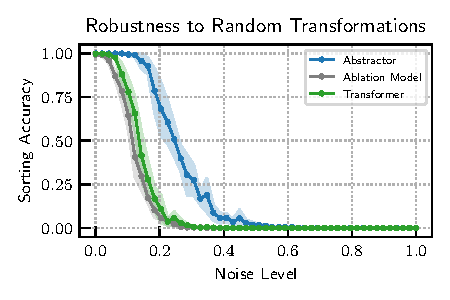
\includegraphics[scale=.95]{figures/experiments/additive_robustness.pdf}
        \vskip-5pt
        \caption{The Abstractor is more robust to corruption by additive noise. }\label{fig:exp_robustness1}
    \end{subfigure}\hspace{\fill}
    \begin{subfigure}[t]{0.40\textwidth}
        %\centering
        \hskip-.6in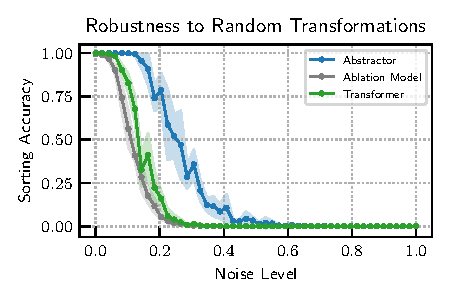
\includegraphics[scale=.95]{figures/experiments/multiplicative_robustness.pdf}
        \vskip-5pt
        \caption{The Abstractor is more robust to corruption by a random linear transformation.}\label{fig:exp_robustness2}
    \end{subfigure}
    \caption{Experiments on robustness.}\label{fig:exp_robustness}
\end{figure}
% 
%\newcommand{\MLP}{\text{MLP}}
%\newcommand{\FeedForward}{\text{FeedForward}}
%\newcommand{\Softmax}{\text{Softmax}}
%\newcommand{\reals}{\mathbb{R}}
\def\m{m}


\section{Relational symbolic message-passing}
\label{sec:message_passing}

At a high level, the primary function of a relational abstractor is to compute abstract relational features of its
inputs. That is, given a set of input objects $o_1, \ldots, o_\m$, the relational abstractor computes a function on
the set of pairwise relations between objects $\{ R(o_i, o_j) \}_{i,j}$, where $R(\cdot, \cdot)$ is a relation between a pair of objects; the relations are learned to carry out a specific prediction task,
% JDC ADDITION:
in such a form that they can be generalized to any arbitrarily large set of inputs that are appropriate for the task.

At the core of relational abstractors is an operation we refer to as \textit{relational symbolic message-passing}.
The input to this operation is a relation tensor $R = \left[R(o_i, o_j)\right]_{i,j=1}^\m$, where $R(o_i, o_j) \in \mathbb{R}^{d_r}$ is a vector describing the relation between object $o_i$ and object $o_j$. We will come back to how an abstractor computes the relation tensor,
% JDC ?OK:
after considering how the symbols on which it operates can be learned.

The first set of learnable parameters of symbolic message-passing is a set of symbols $s_1, \ldots, s_\m \in \mathbb{R}^{d_s}$, where the hyperparameter $d_s$ is the dimension of the symbolic vectors. We call these parameters \textit{symbols} because each of them references (or ``is bound to") a particular object, but they are independent of the values of these objects. That is, the $i$th symbol references the $i$th object, but the value of $s_i$ is independent of the value of $o_i$. The use of those learned input-indpendent symbols is how symbolic message-passing achieves its abstraction.

In relational symbolic message-passing, we perform message-passing on these learned symbolic parameters according to the relation tensor $R$. In general, this message-passing operation can be described as a set-valued function of the form
\begin{equation}
    \label{eq:symbolic_message_passing}
    s_i \leftarrow \text{Update}\Big( s_i, \ \left\{ \left(R[i,j], s_j\right)\right\}_{j\in[m]}\Big), \quad i = 1, \ldots, m
\end{equation}
That is, the value of the $i$th symbol is updated as a function of the set of tuples $(R[i,j], s_j)$ of the relations with all other objects and the symbols of these objects. The symbols $s_j$ are naturally viewed
as values on the nodes of a graph, and the relations $R[i,j]$ are naturally viewed as weights on the edges. A simple but important special case of this is
\begin{equation}
    \label{eq:linear_symbolic_mp}
    s_i \leftarrow \sum_{j=1}^{m} R[i,j] s_j, \quad i=1, \ldots, m
\end{equation}
In the above, suppose that $d_r = 1$. Otherwise, the above operation is done for each dimension of the relation $R$ and the result is concatenated, as in multi-head attention.

Following message-passing, each updated symbol $s_i$, can be passed through a feedforward neural network $f:\reals^{d_s}\rightarrow \reals^{d_s}$ to compute a non-linear function of the output. %Empirically, a residual connection and layer normalization may be useful, as in a transformer.
This message-passing operation can be repeated multiple times to iteratively update the symbolic vectors.  The output of relational symbolic message-passing is the set of symbols $A$ at the end of this sequence of message-passing operations. The overall procedure is summarized in Algorithm~\ref{alg:relational_abstractor}. In Section~\ref{sec:function_spaces} we characterize the class of functions on relations that this operation can compute.

% JDC: Shouldn't $d_s$ be included in the list of hyperparameters below?
\begin{algorithm}[th!]
    \caption{Relational Abstractor}\label{alg:relational_abstractor}
    \SetKwFor{For}{for}{do}{end}
    \SetKwInOut{Input}{Input}
    \SetKwInOut{Output}{Output}
    \SetKwInOut{LearnableParams}{Learnable parameters{\ }}
    \SetKwInOut{HyperParams}{Hyperparameters}

    \Input{Encoder entities: $E = (o_1, \ldots, o_\m) \in \mathbb{R}^{d_e \times m}$}
    \HyperParams{$L$ (number of layers), $H$ (number of heads), feedforward network structure}
    \LearnableParams{Symbols $S \in \reals^{d_s \times m}$, parameters $\{\theta_l\}$ of attention heads and feedforward models}
    \Output{Abstracted sequence: $A = (a_1, \ldots, a_\m) \in \reals^{d_a \times m}$}
    \vspace{1em}

    $A \gets S$

    \For{$l \gets 1$ \KwTo $L$}{
        $A \gets \text{SelfAttention}_{\theta_l}(A)$\;
        $A \gets \crossattend{E}{E}{A}{\theta_l}$\;
        $A \gets\FeedForward_{\theta_l}(A)$\;
        }
\end{algorithm}

\subsection{Computing the relation tensor with relational cross-attention}

Symbolic message passing is the first of the two main
%ingredients
components
of abstractors. What remains is to describe how the abstractor computes the relation tensor $R$. This is
done through a variant of transformer cross-attention that we refer to as \textit{relational cross-attention}.
To motivate this, we first describe how we can compute relations between pairs of objects through inner products.
The inner product operation is a natural way to capture notions of relations and similarity. In Euclidean space,
inner products capture the geometric alignment between vectors. Similarly, for objects with vector representations,
inner products between these vector representations can capture relations between these objects.

In general, we can formulate inner product relations as the standard Euclidean inner product between a pair of transformed object vectors. That is, 
\begin{equation}
    R(o_i, o_j) = \langle \phi(o_i), \psi(o_j) \rangle
    \label{eq:relation_innerproduct}
\end{equation}
This captures a large class of relation functions. In particular, the theory of reproducing kernel Hilbert spaces implies that any continuous, symmetric function on pairs of objects can be approximated with such functions
\citep{universal}. Multi-dimensional relation functions can be achieved by stacking multiple such inner products.
In the next section we frame this explicitly in terms of transformer operations.

% NOTE / TODO: need to describe what we mean by `relations', `relation functions', `inner product relations', etc. in more detail somewhere?
% maybe in intro at high-level
% JDC: I HAD THE SAME INCLINATION ABOVE (IN RESPONSE "The inner product operation is a natural way to capture...).
% ONE THOUGHT WE HAVE HAD IS THAT THEY CAN ALSO BE USED TO CAPTURE CONTRASTIVE RELATIONSHIPS, SINCE THE
% INNER PRODUCT IS SENSITIVE TO THE NORMS OF THE VECTORS (AS LONG AS NO FORM OF NORMALIZATION IS APPLIED, INCLUDING
% SOFTMAX FOR READOUT) -- SIMON CAN TALK ABOUT THIS ON MONDAY.

% comment this out
% \end{document}

% \def\rdot{\bigcdot}
\def\F{{\mathfrak{F}}}
\def\MLP{\text{MLP}}

\section{Function classes}
\label{sec:function_spaces}

In this section, we will discuss the class of relational functions computable by the symbolic message-passing operation in relational abstractors. We also comment on the robustness of these operations. In the process, we characterize the class of relational functions realizable by inner product relational neural networks, which may be of independent interest.

We start by presenting a universal approximation result for inner product relations. This will be useful when characterizing the class of functions computable by abstractors, but is also of interest more generally for relational machine learning.

\subsection{Function class of inner product relations}

A natural way to model relations between objects is through inner products between their vector representations. Consider vectors living in a space \(\mathcal{X}\). We would like to learn a relation function \(R: \mathcal{X} \times \mathcal{X} \to \reals^{d_r}\) which maps pairs of objects in \(\mathcal{X}\) to a \(d_r\)-dimensional vector describing the relation between these objects. We will model this relation function as a vector of inner products between transformations of the objects' representations:
\begin{equation}
	\label{eq:inner_product_relations}
	R(x, y) = \begin{pmatrix}\langle \phi_{1}(x), \phi_{1}(y) \rangle \\ \vdots \\ \langle \phi_{d_r}(x), \phi_{d_r}(y) \rangle \end{pmatrix},
\end{equation}
where \(\phi_{1}, \ldots, \phi_{d_r}\) are learnable transformations corresponding to each dimension of the relation. These transformations can be thought of as \textit{relational filters}. They extract a particular attribute of the objects such that an inner product of the transformed objects indicates the alignment or similarity along this attribute. Having several different filters allows for modeling rich multi-dimensional relations. This is one notable advantage of this formulation over the CoRelNet model \citep{kerg2022neural}, which processes a relation matrix as input to a multi-layer perceptron.

In a deep learning model, a natural choice is for \(\phi_{1}, \ldots, \phi_{d_r}\) to be \(d_r\) different neural networks (e.g.: MLPs, CNNs, etc. depending on the object space \(\mathcal{X}\)). Hence, the parameters of \(R\) are \(\boldsymbol{\theta} = (\theta_{1}, \ldots, \theta_{d_r})\), where \(\theta_{i}\) are the parameters of \(\phi_{i}\).

The following result characterizes the class of inner product relations computable by \eqref{eq:inner_product_relations} when \(\phi_{1}, \ldots, \phi_{d_r}\) are feedforward networks. We make use of Mercer's theorem and universal approximation properties of feedforward networks to obtain a universal approximation result for inner product relational neural networks.


\begin{thm}[Function class of inner product relational neural networks]
	\label{thm:function_class_inner_product_relnn}
	\hphantom{~}

	Consider an inner product relational neural network modeling a \(d_r\)-dimensional relation via inner products of neural networks,
	\begin{equation*}
		\langle x, y \rangle_{\MLP} := \begin{bmatrix}\langle \MLP_{\theta_1}(x), \MLP_{\theta_1}(y) \rangle \\ \vdots \\ \langle \MLP_{\theta_{d_r}}(x), \MLP_{\theta_{d_r}}(y) \rangle\end{bmatrix}.
	\end{equation*}

	Suppose the data lies in a compact Hausdorff space \(\mathcal{X}\) (e.g.: a metric space) with a finite countably additive measure. In particular, \(\mathcal{X}\) can be any compact subset of \(\mathbb{R}^d\).

	Then, \(\langle \cdot, \cdot \rangle_{\MLP}\) is a Mercer kernel along each of the \(d_r\) dimensions.

	Furthermore, for any vector-valued relation function \(R: \mathcal{X} \times \mathcal{X} \to \reals^{d_r}\) which is a Mercer kernel in each dimension, there exists an inner product relational neural network which approximates $R$ arbitrarily closely in the superemum norm (i.e.: uniformly over \((x,y) \in \mathcal{X}\times\mathcal{X}\)). More precisely, for all \(\epsilon > 0\), there exists \(d_r\) neural networks with parameters \(\theta_1, \ldots, \theta_{d_r}\) such that \(\sup_{x,y \in \mathcal{X}}{\lVert R(x,y) - \langle x, y \rangle_\MLP \rVert_\infty} < \epsilon\).
\end{thm}

\begin{proof}
	\hphantom{~}

	Denote the given relation function \(R\) by its \(d_r\) components:
	\begin{equation}
		R(x,y) = (R_1(x,y), \ldots, R_{d_r}(x,y)).
	\end{equation}
	By assumption, \(R_i\) is a Mercer kernel for each \(i = 1, \ldots, d_r\). Consider the component \(R_i\). By Mercer's theorem \citep{mercerFunctionsPositive1909, sunMercerTheorem2005, universal}, there exists \((\psi_i)_{i \in \mathbb{N}}\), \(\lambda_i \geq 0\) such that \(R_i(x,y) = \sum_{i=1}^{\infty}{\lambda_i \psi_i(x) \psi_i(y)}\), where \(\psi_i\) and \(\lambda_i\) are eigenfunctions and eigenvalues of the integral operator

	\begin{align*}
		T_R&: L_2(\mathcal{X}) \to L_2(\mathcal{X}) \\
		T_R(f) &= \int_{\mathcal{X}}{R(\cdot, x) f(x) dx}.
	\end{align*}

	Furthermore, the convergence of the series is uniform:
	\begin{equation}
		\lim_{n \to \infty} \sup_{x,y \in \mathcal{X}} \lvert R_i(x,y) - \sum_{j=1}^{n}{\lambda_j \psi_j(x) \psi_j(y) \rvert} = 0
	\end{equation}

	Let \(\tilde{n}_i\) be such that
	\begin{equation}
		\label{eq:proof_mercer_thm_unif_abs_cv}
		\sup_{x,y \in \mathcal{X}} \left\lvert R_i(x,y) - \sum_{j=1}^{n}{\lambda_j \psi_j(x) \psi_j(y)} \right\rvert < \frac{\epsilon}{2}
	\end{equation}

	Now, for \(j = 1, \ldots, \tilde{n}_i\), let the \(i\)th neural network with parameters \(\theta_i\) be a function from \(\mathcal{X}\) to \(\tilde{n}_i\)-dimensional space. Let \((\sqrt{\lambda_1} \psi_1, \ldots, \sqrt{\lambda_{\tilde{n}_i}} \psi_{\tilde{n}_i})\) be the function to be approximated by the \(i\)th neural network. By the universal approximation property of neural networks, for any \(\epsilon_1\), there exists a neural network with parameters \(\hat{\theta}_i\) such that
	\begin{equation}
		\label{eq:proof_NN_UAP}
		\sup_{x\in \mathcal{X}}{\left\lvert (\MLP(x))_j - \sqrt{\lambda_j} \psi_j(x) \right\lvert } < \epsilon_1
	\end{equation}

	We refer to \citep{hornikMultilayerFeedforward1989, cybenkoApproximationSuperpositions1989, barronUniversalApproximation1993} for results guaranteeing the existence of neural networks which can approximate any continuous function over a bounded domain.

	For ease of notation, we denote \(\MLP_{\hat{\theta}_i}\) simply by \(\MLP\), omitting the dependence on fixed \(i\). Furthermore, \(\MLP(x)_j\) is the \(j\)th component of the output of \(\MLP(x)\). Now note that the approximation error for \(R_i\) is bounded by
	\begin{equation}
		\label{eq:proof_approx_bound}
		\begin{split}
			\sup_{x, y \in \mathcal{X}}&{
				\left\lvert R_i(x,y) - \langle \MLP(x), \MLP(y) \rangle \right\rvert}\\
			&= \sup_{x, y \in \mathcal{X}}{
				\left\lvert R_i(x,y) - \sum_{j=1}^{\tilde{n}_i}{\MLP(x)_j \MLP(y)_j} \right\rvert} \\
			&\leq \sup_{x,y \in \mathcal{X}}{ \left(
				\left\lvert R_i(x,y) - \sum_{j=1}^{\tilde{n}_i}{\lambda_j \psi_j(x) \psi_j(y)} \right\rvert
				+ \left\lvert \sum_{j=1}^{\tilde{n}_i}{\lambda_i \psi_j(x) \psi_i(y) - \MLP(x)_j \MLP(y)_j} \right\rvert  \right) }
		\end{split}
	\end{equation}
	The first term is less than \(\frac{\epsilon}{2}\) by \eqref{eq:proof_mercer_thm_unif_abs_cv}. The second term can be bounded uniformly on \(x,y\) by
	\begin{equation*}
		\begin{split}
			&\left\lvert \left(\sum_{j=1}^{\tilde{n}_i}{\lambda_i \psi_j(x) \psi_i(y)}\right) - \langle \MLP(x), \MLP(y) \rangle \right\rvert  \\
			&\leq \sum_{j=1}^{\tilde{n}_i}{ \left\lvert \lambda_i \psi_j(x) \psi_i(y) - \MLP(x)_j \MLP(y)_j \right\rvert} \\
			&\leq \sum_{j=1}^{\tilde{n}_i}{\left(
				\left\lvert \MLP(x)_j \right\rvert \left\lvert \sqrt{\lambda_j} \psi_j(y) - \MLP(y)_j \right\rvert
				+ \lvert \MLP(y)_j \rvert \left\lvert \sqrt{\lambda_j} \psi_j(x) - \MLP(x)_j \right\rvert
				\right)}
		\end{split}
	\end{equation*}
	Let \(\epsilon_1\) in \eqref{eq:proof_NN_UAP} be small enough such that the above is smaller than \(\frac{\epsilon}{2}\). 	Then, by \eqref{eq:proof_approx_bound}, we have that
	\begin{equation*}
		\sup_{x, y \in \mathcal{X}}{
			\lvert R_i(x,y) - \langle \MLP(x), \MLP(y) \rangle \rvert} \leq \frac{\epsilon}{2} + \frac{\epsilon}{2} = \epsilon
	\end{equation*}

	We repeat this for each component of the relation function \(R_i\), \(i=1, \ldots, d_r\), obtaining \(d_r\) neural networks each with parameters \(\hat{\theta}_i\). Thus, \(\sup_{x,y \in \mathcal{X}}{\lVert R(x,y) - \langle x, y \rangle_\MLP \rVert_\infty} < \epsilon\).
\end{proof}

\begin{remark}
	The result also holds for universal approximators other than feedforward neural networks, with a nearly identical proof.
\end{remark}

\Cref{thm:function_class_inner_product_relnn} shows that an inner product relational neural network can approximate arbitrary continuous, symmetric, positive semi-definite relation functions \(R(\cdot, \cdot)\). We now make a couple of remarks.

Learning the relation function in equation \eqref{eq:inner_product_relations} involves learning \(d_r\) different non-linear transformations \(\phi_{1}, \ldots, \phi_{d_r}\). To enable greater weight-sharing, we can instead have a single non-linear learned function \(\phi: \mathcal{X} \to \mathbb{R}^{\tilde{d}}\) along with \(d_r\) linear projections \(W_k \in \mathbb{R}^{m \times \tilde{d}}\), such that
\begin{equation}
	\label{eq:weight_sharing_inner_product_relnn}
	R(x,y) = \begin{pmatrix}\langle W_1 \phi(x), W_1 \phi(y) \rangle \\ \vdots \\ \langle W_{d_r}\phi(x), W_{d_r}\phi(y) \rangle\end{pmatrix}.
\end{equation}
This is does not shrink the class of computable relation functions since for any set of learned functions \(\phi_1, \ldots, \phi_{d_r}\) in the former set up, we can consider a single \(\phi\) which is simply a concatenation of all these outputs and have the linear projections extract the appropriate components.

Additionally, we can consider inner products of the form
\begin{equation}
	\label{eq:nonsymmetric_inner_product_relnn}
	\langle W_k^{(1)} \phi(x_i), W_k^{(2)} \phi(x_j) \rangle,
\end{equation}
\noindent where the linear projections for the first and second entities may be different, in order to achieve non-symmetric relation functions. This yields a strictly larger class of relation functions than in Theorem \ref{thm:function_class_inner_product_relnn}.

This is closely related to the cross-attention operation in transformers (and  abstractors). In cross-attention, the relation between two objects is given by an inner product between the two object vectors transformed by a `query' matrix and a `key' matrix respectively: \(\langle W_Q x, W_K y \rangle\). A `relation tensor' giving pairwise relations is then computed as \(\Softmax((W_K X)^\top (W_Q X))\), where \(X = \begin{bmatrix} x_1 & \cdots & x_\m\end{bmatrix}\) are the object vectors. The multiple heads of multi-head attention similarly correspond to the multi-dimensional relations modeled by the transformations \(\phi_{1}, \ldots, \phi_{d_r}\) in the inner product relational neural network \ref{eq:inner_product_relations}.

\begin{remark}
	The function class of non-symmetric inner product relational neural networks of the form
	\[ R(x,y) = \begin{pmatrix}
		\langle \phi_1(x), \psi_1(y) \\
		\vdots \\
		\langle \phi_{d_r}(x), \psi_{d_r}(y)
	\end{pmatrix}\]
	can also be characterized.
\end{remark}

\subsection{Class of relational functions computable by symbolic message-passing}
\label{ssec:function_class_symbolic_mp}
For the purposes of this analysis, the algorithmic description of symbolic message-passing is presented in \Cref{alg:symbolic_mp}. It is slightly simpler than the algorithmic description of the full relational  abstractor in \Cref{alg:relational_abstractor}---the primary difference is that we omit self-attention between symbolic states.

\begin{algorithm}[ht!]
	\caption{Symbolic Message-Passing}\label{alg:symbolic_mp}
	\SetKwInOut{Input}{Input}
	\SetKwInOut{Output}{Output}
	\SetKwInOut{LearnableParams}{Learnable parameters{\ }}
	\SetKwInOut{HyperParams}{Hyperparameters}

	\Input{Relation tensor: \(R \in \mathbb{R}^{n \times \m \times d_r}\)}
	\HyperParams{\(L\) (number of steps/layers), hyperparameters of feedforward networks}
	\LearnableParams{symbols \(\boldsymbol{s} = (s_1, \ldots, s_\m) \in \reals^{d_s \times \m}\), feedforward neural networks \(\phi^{(1)}, \ldots, \phi^{(L)}\)}
	\Output{Abstracted sequence: \(\boldsymbol{a} = (a_1, \ldots, a _\m) \in \reals^{d_a \times \m}\)}
	\vspace{1em}

	\(A \gets S\)

	\For{\(l \gets 1\) \KwTo \(L\)}{
		\(a_i \gets \sum_{j=1}^{n} R[i,j] a_j, \quad i = 1, \ldots, n\)

		\(a_i \gets \phi^{(l)}(a_i), \quad i = 1, \ldots, n\)
	}
\end{algorithm}



From equation \eqref{eq:linear_symbolic_mp}, the symbolic message-passing operation is clearly bijective as a function on the input relation tensor \(R\), for an appropriate choice of the symbol parameters \(S = (s_1,\ldots, s_\m)\). For example, choosing \(S = I_{\m \times \m}\) (i.e.: the \(i\)th symbolic vector is the indicator \(\m\)-vector with a \(1\) in the \(i\)th position, \(s_i = e_i\)) reproduces the relation tensor after one message-passing operation:
\begin{equation*}
	s_i  \leftarrow  \sum_{j=1}^{n} R[i,j] e_j = \begin{pmatrix}R[i,1] \\ R[i,2] \\ \vdots \\ R[i,n]\end{pmatrix}.
\end{equation*}
More generally, one linear step of symbolic message-passing yields updated symbolic vectors such that \(s_i'\) is a linear function of the vector of all objects' relations with object \(i\):
\begin{equation*}
	s_i \leftarrow = S \begin{pmatrix}R[i,1] \\ \vdots \\ R[i,n]\end{pmatrix}.
\end{equation*}
Following the linear step in symbolic message-passing, each updated symbolic state is transformed via a neural network. Hence, the \(i\)th abstracted value after symbolic message-passing is given by
\begin{equation*}
	a_i = \phi\left(S r_i \right),
\end{equation*}
where \(\phi\) is a neural network, and \(R_i\) is the vector of object \(i\)'s relations with every other object, \(R_i = \begin{pmatrix}R[i,1] & \cdots & R[i,n]\end{pmatrix}^\top\). Hence, \(a_i\) summarizes all the information about object \(i\)'s relations to all other objects. We summarize this discussion by the following
lemma, which follows from universal approximation properties of feed-forward networks.

\begin{lemma}
	\label{lemma:function_class_1_step_symbolic_mp}
	A one-step symbolic message-passing operation (in \Cref{alg:symbolic_mp}) can compute arbitrary functions of a each object's relations with other objects in the input sequence. That is, there exists a choice of symbols \(s_1, \ldots, s _\m\) and parameters of the feed-forward network such that \(a_i\) computes an arbitrary function of object \(i\)'s relations, \(r_i = \begin{pmatrix}R[i,1] & R[i,2] & \cdots & R[i,n]\end{pmatrix}^\top\).
\end{lemma}


Thus, the abstracted sequence after a single step of symbolic message-passing has the form
\begin{equation}
	\label{eq:abstracted_seq_1_layer_abstractor}
	A^{(1)} = (a_1^{(1)}, \ldots, a_\m^{(1)}) = \left(\phi(r_1), \phi(r_2), \ldots, \phi(r_\m)\right),
\end{equation}
where \(\phi\) is an arbitrary learnable function shared by all abstracted objects, and \(r_i\) is the vector of object \(i\)'s relations with every other object.

That is, \(a_i^{(1)}\) summarizes object \(i\)'s relations with other objects. With further symbolic message-passing operations, the \(i\)th abstracted vector can be made to represent information about other relations, not necessarily involving the \(i\)th object. For example, at the second layer, the abstracted vectors take the form
\begin{equation}
	a_i^{(2)} = \phi^{(2)} \left( \sum_{j=1}^{n} R[i,j] a_j^{(1)} \right) = \phi^{(2)} \left( \sum_{j=1}^{n} R[i,j] \phi^{(1)}(R_j) \right).
\end{equation}

We conclude this subsection by remarking that the above analysis concerns \Cref{alg:symbolic_mp}---a simplified version of the relational  abstractor. In particular, while it captures the effects of relational cross-attention, it does not include self-attention on the abstract symbols. The analysis indicates that we should expect the function class generated by a relational  abstractor module in \Cref{alg:relational_abstractor} to be no smaller than that of the simple symbolic message-passing in \Cref{alg:symbolic_mp}.


\subsection{Composing  abstractors to compute relations on relations}
\label{ssec:compsing_abstractors}

As described in \Cref{sec:abstractors_as_transformer_modules}, the abstactor framework supports composing  abstractors in the form
\begin{equation*}
	\texttt{Encoder} \to \texttt{Abstractor} \to \cdots \to \texttt{Abstractor} \to \texttt{Output}
\end{equation*}
Here, we analyze the function class generated by a composition of several abstractors. We make the simplifying assumption that each single layer abstractor takes the simplified form of the symbolic message-passing operation in \Cref{alg:symbolic_mp}. This corresponds to omitting the self-attention operation in \Cref{alg:relational_abstractor} while maintaining the relational cross-attention with the sequence of output vectors at the previous  abstractor.

We saw in the previous section that a one-layer abstractor is able to compute arbitrary functions  of each object's relations. Observe that the output sequence of abstracted objects is a sequence of `relational vectors'. That is, objects which summarize relational information. Hence, chaining together a sequence of  abstractors allows the computation of relations on relations.

% TODO: formalize or refine presentation of result
\begin{lemma}
	\label{lemma:function_class_composed_abstractors}
	A chain of \(k\) single-layer  abstractors is able to compute arbitrary ``\(k\)th order relational functions'' in the sense of the proof below.
\end{lemma}
\begin{proof}[Proof sketch]
	In \Cref{ssec:function_class_symbolic_mp} we characterized the output of a 1-layer abstractor as
	\begin{equation*}
		A^{(1)} = (a_1^{(1)}, \ldots, a_\m^{(1)}) = \left(\phi^{(1)}(r_1), \phi^{(1)}(r_2), \ldots, \phi^{(1)}(r_\m)\right),
	\end{equation*}
	Note that we will now use the superscript to denote the abstractor in the chain rather than the layer depth in a single  abstractor, as all  abstractors have a depth of one.

	Let the second abstractor's symbols be denoted by \(S^{(2)} = (s_1^{(2)}, \ldots, s_\m^{(2)})\). Then,
	\begin{equation*}
		a_i^{(2)} = S^{(2)} \begin{bmatrix}R^{(2)}[i,1] \\ \vdots \\ R^{(2)}[i,n]\end{bmatrix},
	\end{equation*}
	where,
	\begin{equation*}
		R^{(2)} = \Softmax\left((W_K A^{(1)})^\top (W_Q A^{(1)})\right).
	\end{equation*}
	Observe that
	\begin{equation*}
		\left[(W_K A^{(1)})^\top (W_Q A^{(1)})\right]_{ij} = \langle W_Q \phi^{(1)}(r_j), W_K \phi^{(1)}(r_i) \rangle.
	\end{equation*}
	By Theorem \ref{thm:function_class_inner_product_relnn}, composing an arbitrary learnable function \(\phi\) with inner products enables learning arbitrary relation functions on the input space (i.e.: any continuous, symmetric, positive semi-definite bivariate function. Here, the class of functions is actually larger since it allows for non-symmetric relation functions when \(W_Q \neq W_K\)).

	In the above, the space over which we are computing relations is itself a space of relation vectors. That is, \(\langle W_Q \phi^{(1)}(R_j), W_K \phi^{(1)}(R_i) \rangle\) computes a relation between object \(i\)'s relations and object \(j\)'s relations. Hence, choosing \(s_i^{(2)} = e_i\) and ignoring the Softmax for now, yields
	\begin{equation*}
		a_i^{(2)} = \phi^{(2)}\left(\begin{bmatrix}\langle W_Q \phi^{(1)}(r_i), W_K \phi^{(1)}(r_1) \rangle \\ \vdots \\ \langle W_Q \phi^{(1)}(r_i), W_K \phi^{(1)}(r_\m) \rangle\end{bmatrix}\right).
	\end{equation*}
	Thus, \(a_i^{(2)}\) computes arbitrary second-order relation functions. Namely, it computes arbitrary relations between object \(i\)'s relation vector and every other object's relation vector.

	More generally, at layer \(l\), we have
	\begin{align*}
		R^{(l)} &= \Softmax\left((W_K A^{(l-1)})^\top (W_Q A^{(l-1)})\right),\\
		a_i^{(l)} &= \phi^{(l)}\left(S^{(l)} \begin{bmatrix}R^{(l)}[i,1] \\ \vdots \\ R^{(l)}[i,n]\end{bmatrix}\right).
	\end{align*}
	Thus, \(R^{(l)}\) computes \(l\)th order-relations, and \(a_i^{(l)}\) is a linear map applied to the \(l\)th-order relations involving object \(i\).
\end{proof}


\subsection{Robustness and error correction}

For the relational cross-attention mechanism used by abstrators, an \(m\times m\) relation
is computed as  \(R = \mbox{Softmax}(K^T Q)\)
and relational cross attention then transforms the symbols by
\(A = SR\) so that each abstract variable \(a_j\) is in the convex hull of the set of symbols.
As long as \(S\) has rank \(m\), relations are uniquely determined from the abstract symbols.
Here we point out how the transformed symbols can be robust to noise if the symbols are
sufficiently redundant.

Specifically, suppose that the symbols \(S\) are transformed to \(A\) and corrupted with additive noise:
\begin{equation}
  A = SR + \Xi
\end{equation}
where a fraction \(\epsilon\) of the entries of \(\Xi\) are drawn from an adversarial noise distribution, and the other entries are zero; dropout noise is also possible.
This can be studied as an instance of compressed sensing and ``model repair'' \citep{candes_randall,model_repair}.  In particular, the relations can be recovered using the  robust regression estimator
\begin{equation}
  \hat r_j = \argmin_{u \in\reals^m} \| a_j - S u\|_1 \label{eq:lp}
\end{equation}
where \(A = (a_1,a_2,\ldots, a_m)\) with columns \(a_j\in\reals^d\).
The main lemma in \cite{model_repair} states that the following two conditions suffice:

\underline{Condition A:}
  There exists some \(\sigma^2\), such that for any fixed \(c_1,...,c_d\) satisfying \(\max_i|c_i|\leq 1\),
  \begin{equation}
    \left\|\frac{1}{d}\sum_{i=1}^d c_i s_{i\rdot} \right\|^2\leq \frac{\sigma^2 m}{d},
  \end{equation}
with high probability, where \(s_{i\rdot}\in\reals^m\) is the \(i\)th row of \(S\).

\underline{Condition B:}
  There exist \(\underline{\kappa}\) and \(\overline{\kappa}\), such that
  \begin{eqnarray}
  \label{eq:l1-upper-A} \inf_{\|\Delta\|=1}\frac{1}{d}\sum_{i=1}^d|s_{i\rdot}^T\Delta| &\geq& \underline{\kappa}, \\
  \label{eq:l2-upper-A} \sup_{\|\Delta\|=1}\frac{1}{d}\sum_{i=1}^d|s_{i\rdot}^T\Delta|^2 &\leq& \overline{\kappa}^2,
  \end{eqnarray}
  with high probability.

\begin{thm}\label{thm:main-improved}
  Assume the symbol matrix \(S\) satisfies Condition A and Condition B. Then if
  \begin{equation}
  \frac{\overline{\kappa}\sqrt{\frac{m}{d}\log\left(\frac{e d}{k}\right)}+\epsilon\sigma\sqrt{\frac{m}{d}}}{\underline{\kappa}(1-\epsilon)}
  \end{equation}
  is sufficiently small, the linear program \eqref{eq:lp} recovers \(R\), so that \(\hat r_j = r_j\) with high probability.
  \end{thm}

The condition is essentially that
  \begin{equation}
    \frac{1}{1-\epsilon} \sqrt{\frac{m}{d}}
  \end{equation}
  is small, meaning that the dimension \(d\) of the symbols needs to be sufficiently large relative
  to the dimension \(k\) of the relation.

  \subsection{Sparse, high-dimensional relations}

 The above setting ensures enough redundancy to recover the relations, constraining the number of symbols \(k\) to be small relative to the symbol dimension \(d\). This is not appropriate in the situation where the relations are over a large number \(m\) of elements, for example, the contents of the entire episodic memory.
 In this setting we assume that the relation tensor \(R \in \reals^{m\times m}\) is sparse; that is,
 each column \(r_j \in \Delta_m\) has at most \(k\) nonzero entries: \(\|r_j\|_0 \leq k\). To recover the relation
 we now use the robust lasso estimator, which is a related linear program
\begin{equation}
  \hat r_j = \argmin_{u \in\reals^m} \| a_j - S u\|_1 + \lambda\|u\|_1. \label{eq:rlasso}
\end{equation}
Here we have an analogous theorem, stating that if
\begin{eqnarray}
  \frac{\overline{\kappa}/\underline{\kappa}}{1-\epsilon}\sqrt{\frac{k}{d}\log(2m)}\leq c,
\end{eqnarray}
for some sufficiently small constant \(c>0\), the robust lasso estimator \eqref{eq:rlasso} satisfies
\begin{equation}
  \|\hat r_j - r_j\| \leq C \frac{\overline{\kappa}/\underline{\kappa}^2}{1-\epsilon} \sqrt{\frac{\sigma^2 k}{d} \log(2m)}
\end{equation}
for some constant \(C\).
This implies that we can accurately recover the relation tensor in the high dimensional setting, even when many of the entries of the transformed abstract symbols are corrupted.


The above discussion shows how the relation tensor can be recovered from the transformed symbols, even under adversarial noise, assuming there is sufficient redundancy in the symbols. This implies that it is possible to predict as well from the transformed symbols as from the relations, without explicitly recovering the relations.
Using ideas from \citep{surfing,HandV17}, it may be possible to extend this theory to nonlinear mappings
\(y = \varphi(Au) + \eta\) where \(\varphi(\cdot)\) is an activation function.
%; this could serve as an alternative to the Hopfield model of memory retrieval and pattern completion.


% \section{Code for experiments}
\label{sec:code}

The supplementary material includes code for the experiments reported in \Cref{sec:experiments} of the paper. This code includes Python (Jupyter) notebooks for individual experiments as well as scripts that were run on a GPU cluster to parallelize across multiple experimental designs.


\setcounter{subsection}{4}
\subsection{SET experiments}

This is a standalone implementation of an Abstractor that learns to classify triples of images of cards according 
to whether or not they form a SET, in an end-to-end fashion. First a convolutional neural network is trained to process the color images of the cards. The images are $70 \times 40$ pixels in size with $4$ color channels. The CNN has two convolutional layers, each with $32$ filters of size $5\times 5$ coupled with a $4\times 4$ max pooling layer. The feature maps are flattened and passed through two dense feedforward layers. The CNN is trained to predict the attribute of each card (one, two three; red, green, purple; empty, solid, striped; oval, diamond, squiggle), as a multi-label classification, and then an embedding of dimension $d=32$ of each card is obtained from the intermediate dense layer. 

Next, Abstractors are trained separately for each of the four attributes (number, color, pattern, shape) to learn same/different relations, where the task is to decide if an input pair of cards is the same or different for that attribute. The cards are encoded using the feature map generated from the CNN. We then use the query and key mappings $W_Q$ and $W_K$ learned for these relations to initialize the relations in a multi-head Abstractor. This Abstractor is then trained on a dataset of triples of cards, half of which form a SET, again representing the cards using the CNN feature maps.

The Abstractor is compared to a baseline model where the attributes and the relations are hand-coded symbolically, the relations are represented as vectors of 12 bits. A two-layer MLP is then trained to decide if the triple forms a SET. The MLP using the symbolic representation can be considered as a lower bound on the performance achievable by the Abstractor. We note that the simple Abstractor makes no use of self-attention or any of the other enhancements such as skip-connections commonly used in Transformers.


\end{document}